% This is paper draft
% edited by Haoruo Peng
% Date: 2013.9.5
\documentclass[10pt, conference, compsocconf]{IEEEtran}
\usepackage{amsmath, amssymb}
\usepackage{color}
\usepackage{graphicx}
\usepackage{bbding}
\usepackage{epstopdf}

\newcommand{\bw}{\mathbf{w}}
\newcommand{\bwep}{\mathbf{w}^{\varepsilon}}
\newcommand{\bwfly}{\tilde{\mathbf{w}}}
\newcommand{\bwavg}{\mathbf{wavg}}
\newcommand{\bu}{\mathbf{u}}
\newcommand{\buprev}{\mathbf{uprev}}
\newcommand{\bp}{\mathbf{p}}
\newcommand{\bq}{\mathbf{q}}
\newcommand{\bxi}{\mathbf{\xi}}
\newcommand{\dotwxb}{{\mathbf{w}}^{\mathbf{T}}\mathbf{x}_{i}+b}
\newcommand{\sumt}{\sum_{t=1}^{T} }
\newcommand{\lc}{\left(}
\newcommand{\rc}{\right)}
\newcommand{\li}{\lc i\rc}
\newcommand{\lj}{\lc j\rc}
\newcommand{\tspace}{\hspace*{2em}}
\newcommand{\tspaces}{\hspace*{1.5em}}
\newcommand{\comment}{\textcolor{red}}
\newcommand{\ti}[1]{\tilde{#1}}
\newcommand{\indep}{{\;\bot\!\!\!\!\!\!\bot\;}}

\def\A{{\bf A}}
\def\a{{\bf a}}
\def\B{{\bf B}}
\def\C{{\bf C}}
\def\c{{\bf c}}
\def\D{{\bf D}}
\def\d{{\bf d}}
\def\E{{\bf E}}
\def\e{{\bf e}}
\def\f{{\bf f}}
\def\K{{\bf K}}
\def\H{{\bf H}}
\def\G{{\bf G}}
\def\I{{\bf I}}
\def\R{{\bf R}}
\def\X{{\bf X}}
\def\Y{{\bf Y}}
\def\Q{{\bf Q}}
\def\s{{\bf s}}
\def\S{{\bf S}}
\def\x{{\bf x}}
\def\y{{\bf y}}
\def\z{{\bf z}}
\def\Z{{\bf Z}}
\def\M{{\bf M}}
\def\m{{\bf m}}
\def\n{{\bf n}}
\def\U{{\bf U}}
\def\u{{\bf u}}
\def\V{{\bf V}}
\def\v{{\bf v}}
\def\W{{\bf W}}
\def\w{{\bf w}}
\def\0{{\bf 0}}
\def\1{{\bf 1}}

\def\AM{{\mathcal A}}
\def\FM{{\mathcal F}}
\def\TM{{\mathcal T}}
\def\UM{{\mathcal U}}
\def\XM{{\mathcal X}}
\def\YM{{\mathcal Y}}
\def\NM{{\mathcal N}}
\def\OM{{\mathcal O}}
\def\IM{{\mathcal I}}
\def\GM{{\mathcal G}}
\def\RB{{\mathbb R}}

\def\tx{\tilde{\bf x}}
\def\ty{\tilde{\bf y}}
\def\tz{\tilde{\bf z}}
\def\hd{\hat{d}}
\def\HD{\hat{\bf D}}
\def\hx{\hat{\bf x}}

\def\alp{\mbox{\boldmath$\alpha$\unboldmath}}
\def\bet{\mbox{\boldmath$\beta$\unboldmath}}
\def\epsi{\mbox{\boldmath$\epsilon$\unboldmath}}
\def\etab{\mbox{\boldmath$\eta$\unboldmath}}
\def\ph{\mbox{\boldmath$\phi$\unboldmath}}
\def\pii{\mbox{\boldmath$\pi$\unboldmath}}
\def\Ph{\mbox{\boldmath$\Phi$\unboldmath}}
\def\Ps{\mbox{\boldmath$\Psi$\unboldmath}}
\def\tha{\mbox{\boldmath$\theta$\unboldmath}}
\def\Tha{\mbox{\boldmath$\Theta$\unboldmath}}
\def\muu{\mbox{\boldmath$\mu$\unboldmath}}
\def\Si{\mbox{\boldmath$\Sigma$\unboldmath}}
\def\Gam{\mbox{\boldmath$\Gamma$\unboldmath}}
\def\Lam{\mbox{\boldmath$\Lambda$\unboldmath}}
\def\De{\mbox{\boldmath$\Delta$\unboldmath}}
\def\vps{\mbox{\boldmath$\varepsilon$\unboldmath}}

\def\Ncal{\mathcal{N}}
\def\argmax{\mathop{\rm argmax}}
\def\argmin{\mathop{\rm argmin}}

\def\sgn{\mathrm{sgn}}
\def\tr{\mathrm{tr}}
\def\rk{\mathrm{rank}}
\def\diag{\mathsf{diag}}
\def\vect{\mathsf{vec}}
\def\etal{{\em et al.\/}\,}

\begin{document}

\title{Learning for Logistic Regression Model in Parallel}

\author{
\IEEEauthorblockN{Haoruo Peng}
\IEEEauthorblockA{HTC Research Lab\\Beijing, China\\penghaoruo@hotmail.com}
\and
\IEEEauthorblockN{Ding Liang}
\IEEEauthorblockA{HTC Research Lab\\Beijing, China\\Ding\_Liang@htc.com}
\and
%\IEEEauthorblockN{Deli Zhao}
%\IEEEauthorblockA{HTC Research Lab\\Beijing, China\\zhaodeli@gmail.com}
%\and
\IEEEauthorblockN{Cyrus Choi}
\IEEEauthorblockA{HTC Research Lab\\Beijing, China\\Cyrus\_Choi@htc.com}
\and
\IEEEauthorblockN{Edward Y. Chang}
\IEEEauthorblockA{HTC Research Lab\\Beijing, China\\Edward\_Chang@htc.com}
}

\maketitle

\begin{abstract}
Logistic regression (LR) model has various applications in machine learning.
LR is a supervised learning model for pattern classification and enjoys the benefits of statistical principles.
This paper addresses the issue of computational efficiency for solving LR in big data scenario.
We compare the performance between different computing platforms and different parallel algorithms.
Our goal is to provide valuable suggestions on choosing computing platforms and learning algorithms according to different application situations for specific datasets and machine resources.
We also present a novel parallel sublinear method to optimize the solution of LR.
Overall, two different parallel computing platforms along with three different types of parallel algorithms are carefully studied in this paper.
To enhance capability, we consider the tradeoff between efficiency and accuracy.
Extensive experimental results verify the effective performance of proposed algorithms.
\end{abstract}

\begin{IEEEkeywords}
Logistic Regression Model; Parallel Computing; Sublinear Method; Big Data;
\end{IEEEkeywords}

\section{Introduction} \label{sec:int}
Logistic regression model~\cite{HastieBook:SL} plays a vital role in machine learning.
It is a widely used model in algorithms like PageRank~\cite{page1999pagerank} and anti-spam filtering~\cite{androutsopoulos2000evaluation}.
The model serves for classification problems, and is supported by a substantial body of statistical theories and algorithms.
A binary classification problem modeled by LR can be easily extended to a multi-class classification problem.
Also, due to the strong statistical foundation of the LR model, we can extend achieved results into a deeper analysis which may apply to other classification models. We will focus on the binary LR model in this paper.

In recent years, many modern datasets grow drastically in both data volume and data dimensionality.
Large data volume and high data dimensionality bring unavoidable computational challenges to machine learning problems.
For example, in social networks, we have datasets covering multiple dimensions like friendship relationship and share of common interests. They generally include millions of records over millions of attributes. More evidently, for the task of text and multimedia categorization, we usually have to handle datasets with data volumes in billion scales and each data instance is characterized by thousands of feature dimensions.
We tackle these challenges on both algorithm level and computing platform level via parallelization methods.
For many applications, in order to attain speedup in performance, we can employ not only task parallelism, but also data parallelism~\cite{subhlok1993exploiting}.
In this paper, we mainly discuss issues in task parallelism.

When developing parallel algorithms for LR, it is inevitable to come across the question of choosing which parallel computing platform to employ.
After a thorough survey, we choose two unique and best-known computing platforms to test: Hadoop~\cite{white2012hadoop} and Spark~\cite{zaharia2010spark}.
Hadoop employs HDFS~\cite{borthakur2008hdfs} and MapReduce~\cite{dean2008mapreduce}.
Spark promotes efficiency of iterative algorithms and also supports HDFS.
We will compare design features of these two computing platforms in Section~\ref{sec:platform}.

In sequential optimization algorithms for LR model, a classical way is to resort to stochastic approximation methods.
Stochastic approximation methods, such as stochastic gradient descent~\cite{zhang2004solving} and stochastic dual averaging~\cite{xiao2010dual}, obtain optimal generalization guarantees with a small number of passes over data with runtime linear to the dataset size.
The stochastic gradient descent method can work in an online fashion, as we view sampled data points as data stream over algorithmic iteration.
It is hard to be changed to task-parallelism, but it is blazingly fast.
If we take a step back to the general gradient descent to solve LR model, we can find that it can be actually embarrassingly parallel.
We can take in all of the data at the same iteration and just compute the gradient in a MapReduce fashion.
We can further speed up the runtime by employing sublinear algorithms~\cite{peng2012sublinear} via the application of the stochastic approximation idea.
These methods access a single feature of feature vectors instead of entire feature vectors at each iteration.
We propose a parallel version of this algorithm and achieve the result of comparable accuracy while being faster convergent.

\section{Related Work} \label{sec:rew}

%\subsection{Scalability Solutions}
%
%In big data scenarios, large datasets require us to develop machine learning algorithms towards a more efficient and more parallelized end. Researchers have already done much work to cater for the needs of massive datasets. Early work like Parallel Support Vector Machines (PSVM)~\cite{chang2011psvm} employed an approximation matrix decomposition method based on row selections to reduce memory usage. It can then increase the number of parallel computational nodes to several hundreds. Later, the work of Parallel Latent Dirichlet Allocation (PLDA)~\cite{Liu:2011:PPL:1961189.1961198}~\cite{newman2007distributed} improves the computational efficiency of the LDA model by means of sampling methods. The parallel algorithm in Hadoop is robust, for it has fault tolerance of machine failures, thus taking advantage of Hadoop features. Recently, Dean \etal~\cite{le2011building} claimed that the advantage of parallelization is fully taken in deep learning algorithms. It pushed the limit of parallel computational nodes to a hundred-million level, and in the meantime, achieved the best learning performance ever. GraphLab~\cite{kyrola2012graphchi} is a recently developed tool for large-scale machine learning. It tackles efficiency and scalability problems of machine leaning algorithms by graph-theoretical models.

In this paper, we specifically compares parallelization efforts of LR in two dimensions: platform and algorithm.
\subsection{Computing Platforms}\label{sec:platform}
Two computing platforms that we are working on have their own advantages to implement machine learning algorithms.
The Hadoop~\cite{white2012hadoop} platform allows for distributed processing of large datasets across clusters of computers using simple programming models. It utilizes MapReduce~\cite{dean2008mapreduce} as its computational paradigm, which is easy to be parallelized. In addition, Hadoop provides a Distributed File System (HDFS). Both MapReduce and HDFS are designed to handle node failures in an automatic way, making Hadoop support large clusters that are built on commodity hardware.
Spark~\cite{zaharia2010spark} is a cluster computing system that aims to make data analysis fast. It supports in-memory cluster computing. A job can load data into memory and query it repeatedly by creating and caching resilient distributed datasets (RDDs). Moreover, RDDs achieve fault tolerance through lineage: information about how RDDs are derived from other RDDs is stored in reliable storage, thus making RDDs easy to be rebuilt if a certain partition is lost. Spark can run up to 100 times faster than Hadoop for iterative algorithms.

In Table~\ref{tab:systemcmp}, we compare different features between Hadoop and Spark computing platforms.
For simplicity, we use short abbreviations in the table.
Spark supports two types of operations on RDDs: Actions and Transformations (As and Ts).
Actions include functions like \textit{count}, \textit{collect} and \textit{save}. They usually return a result from input RDDs.
Transformations include functions like \textit{map}, \textit{filter} and \textit{join}. They normally build new RDDs from other RDDs, which comply with the lineage rule.
In the table, we use ``NFS" to represent ``Normal File System" and "Fault Tolerance" here is specifically for node failure situations.
\begin{table}[h]
\centering
\caption{Platform Comparison: Hadoop vs. Spark}\label{tab:systemcmp}\vspace{-0.3cm}
\begin{tabular}{|c|c|c|}
\hline
           & Hadoop & Spark \\
\hline
Computational Paradigm  & MapReduce & As and Ts \\
\hline
File System Supported & HDFS & HDFS and NFS \\
\hline
Design Concept  & Key-value Pairs & RDD \\
\hline
Fault Tolerance Technique & Redundancy & Lineage \\
\hline
\end{tabular}\vspace{-0.5cm}
\end{table}

It is worth mentioning that Apache Mahout~\cite{mahoutscalable} runs on Hadoop, and it is a scalable machine learning library. It integrates many core algorithms for clustering, classification and collaborative filtering in its package. It is highly optimized so that Mahout also has good performance for non-distributed algorithms. We will use it as a baseline in the experiments.

\subsection{Sublinear Methods}
Sublinear methods are recently proposed by many researchers.
Clarkson \etal~\cite{clarkson2010sublinear} first presented the solution of approximation algorithms in sublinear time.
It is applied to optimization problems for linear classifiers and minimum enclosing balls.
The algorithm employs a novel sampling technique along with a new multiplicative update procedure.
Hazan \etal~\cite{hazanbeating} exploited the approach to linear SVM.
Cotter \etal~\cite{cotter2012kernelized} extended the method to kernelized SVM.
%In~\cite{hazan2011optimal}, Hazan \etal applied the sublinear approximation approach to solve linear regression with penalties.
%Garber and Hazan~\cite{garberapproximating} also developed it in Semi-Definite Programming (SDP).
Peng \etal~\cite{peng2012sublinear} utilized the method in the LR model with penalties and developed sequential sublinear algorithms for both $\ell_1$-penalty and $\ell_2$-penalty.

\section{Logistic Regression Model and Sequential Sublinear Algorithm} \label{sec:plr}

\subsection{Logistic Regression Model} \label{sec:def}
In this paper, we are mainly concerned with the binary classification problem.  	
We define the training dataset as $\XM=\{(\x_i, y_i): i=1, \ldots, n\}$, where $\x_i \in \RB^d$ are input samples and $y_i \in \{-1, 1\}$ are the corresponding labels.
For simplicity, we will use the notation $\X=[{\x}_{1}, {\x}_{2}, \ldots, {\x}_n]^{T}$ and $\y=(y_1, y_2, \ldots, y_n)^T$ to represent the training dataset in the following.
To fit in the logistic regression model, the expected value of $y_i$ is given by\vspace{-0.2cm}
\[
P(y_i|\x_i)= \frac{1}{1+ \exp(- y_i(\x_i^T \w + b))} \triangleq g_i(y_i),\vspace{-0.2cm}
\]
where $\w=(w_1, \ldots, w_d)^T \in \RB^d$ is a regression vector and $b\in \RB$ is an offset term.

The learning process aims to optimize $\w$ and $b$.
It is a common practice to add penalties to LR model in order to avoid overfitting and make the optimization result more practical.
Typically, for $\ell_2$-penalty, we solve the following optimization problem:\vspace{-0.2cm}
\begin{equation} \label{eqn:1}
	\max_{\bw ,b} \; \Big\{F(\w, b| \XM) - \frac{\lambda}{2}  \|\bw\|_2^{2} \Big\}.\vspace{-0.2cm}
\end{equation}
For $\ell_1$-penalty, we optimize the following criterion: \vspace{-0.2cm}
\begin{equation} \label{eqn:2}
	\max_{\bw ,b} \;  \big\{F(\w, b|\XM)- \gamma{\|\bw \|}_{1}\big\}.\vspace{-0.2cm}	
\end{equation}
Here, we define $F(\w, b| \XM) = \sum_{i=1}^n \log g_i(y_i)$ in both (\ref{eqn:1}) and (\ref{eqn:2}). To be brief, we omit the derivation here.

\subsection{Sequential Sublinear Algorithm}
We use the following notations to define sequential sublinear algorithm for penalized logistic regression. $clip\lc \cdot \rc$ is a projection function defined as $
clip\lc a,b \rc \triangleq \max \lc \min \lc a,b \rc ,-b\rc,\,a,b\in \mathbb{R}$. $\sgn \lc \cdot \rc$ is the sign function; namely, $\sgn \lc \cdot \rc \in \{-1,0,1\}$.
$g\lc \cdot \rc$ is the logistic function $g \lc x \rc=1/(1+e^{-x})$.

In Algorithm~1, we give the sequential sublinear approximation procedure for logistic regression. The algorithm is mainly from~\cite{peng2012sublinear}. Symbols we use here comply with the definition in Section~\ref{sec:def}. $\varepsilon$ controls learning rate, $T$ determines iteration number, and $\eta$ defines approximation level. Details of the parameter initialization step is studied in~\cite{peng2012sublinear}. To be concise, we omit them in this paper.
	\begin{table} [ht]
	\begin{tabular}{l}
	\hline\noalign{\smallskip}
	\textbf{Algorithm 1}: Sub-Linear Logistic Regression (SLLR) \\
	\noalign{\smallskip}
	\hline
	\noalign{\smallskip}
	1:	Input parameters: $\varepsilon, \nu~or~\gamma, X, Y$ \\
	2:	Initialize parameters: $T, \eta, {\mathbf{u}}_{0}, {\bw}_{1}, {\mathbf{\bq}}_{1}, {b}_{1}$\\
	3:	Iterations: $t=1 \sim T$ \\
	4:	\tspace ${\bp}_{t}\leftarrow{\bq}_{t}/{\|{\bq}_{t}\|}_{1}$ \\
	5:  \tspace Choose ${i}_{t}\leftarrow i$ with probability $\bp(i)$ \\
	6:	\tspace $coef\leftarrow{y}_{{i}_{t}}g\lc-{y}_{{i}_{t}}\lc {{\bw}_{t}}^{T}{\mathbf{x}}_{i_t}+{b}_{t} \rc\rc$ \\
	7:	\tspace ${\bu}_{t}\leftarrow {\bu}_{t-1}+\frac{coef}{\sqrt{2T}}{\mathbf{x}}_{{i}_{t}}$ \\
    8:  \tspace ${\bxi}_{t}\leftarrow \argmax_{\bxi\in \Lambda}\lc{{\bp}_{t}}^{T}\bxi\rc$, if input $\nu$ for $\ell_2$-penalty \\
    9:  \tspace $\bu_t\leftarrow$ soft-thresholding operations, if input $\gamma$ for $\ell_1$-penalty \\
	10:	\tspaces ${\bw}_{t}\leftarrow {\bu}_{t}/\max \left\{1,\|{\bu}_{t}\|_2 \right\}$ \\
    11: \tspaces ${b}_{t}\leftarrow \sgn\lc {{\bp}_{t}}^{T}\mathbf{y}\rc$ \\
	12:	\tspaces Choose ${j}_{t}\leftarrow j$ with probability ${{\bw}_{t}\lj}^{2}/{\|{\bw}_{t}\|_2}^{2} $ \\
	13:	\tspaces Iterations: $i=1 \sim n$ \\
	14:	\tspaces\tspace $\sigma \leftarrow \mathbf{x}_{i} \lc {j}_{t}\rc{\|{\bw}_{t}\|_2}^{2}/{\bw}_{t}\lc {j}_{t} \rc+{\bxi}_{t}\li+{y}_{i}{b}_{t}$ \\
	15:	\tspaces\tspace $\hat{\sigma} \leftarrow clip\lc \sigma,1/\eta \rc$ \\
	16:	\tspaces\tspace ${\bq}_{t+1}\li \leftarrow {\bp}_{t}\li\lc 1-\eta\hat{\sigma} + {\eta}^{2}{\hat{\sigma}}^{2} \rc$ \\
	17:	Output: $\bar{\bw}=\frac{1}{T}\sum_{t}{\bw}_{t},\bar{b}=\frac{1}{T}\sum_{t}{b}_{t}$ \\
	\hline
	\end{tabular} 	
	\label{alg:1}
	\end{table}
Each iteration of the SLLR algorithm has two phases: \textit{stochastic primal update} and \textit{stochastic dual update}.
Steps from line 4 to line 11 consist of the primal part while the dual part is composed of steps from line 12 to line 16.
We give the sublinear algorithm in a unified way for $\ell_2$-penalty and $\ell_1$-penalty.
If we are dealing with $\ell_2$-penalty, we ignore line 9 and accomplish the computation in line 8 by a simple greedy algorithm.
Here, $\Lambda$ represents a Euclidean space with conditions $
\Lambda=\left\{ \bxi\in\mathbb{R}_{n} \, | \, \forall i, \, 0\leq{\xi}_{i}\leq 2, \, {\|\xi \|}_{1}\leq \nu n  \right
\}$.
If we are faced with $\ell_1$-penalty, we ignore line 8 and expand the procedure of line 9 as following.
\begin{table} [ht]
\begin{tabular}{l}
\hline\noalign{\smallskip}
\textbf{Procedure}: Line 9 in Algorithm 1\\
\noalign{\smallskip}
\hline
\noalign{\smallskip}
Iterations: $j=1 \sim d$ \\
\tspace \textbf{if} $\buprev_t\lj>0$ \textbf{and} $\bu_t\lj>0$ \\
\tspace\tspace $\bu_t\lj=\max \lc \bu_t\lj-\gamma ,0 \rc$ \\
\tspace \textbf{if} $\buprev_t\lj<0$ \textbf{and} $\bu_t\lj<0$ \\
\tspace\tspace $\bu_t\lj=\min \lc \bu_t\lj+\gamma ,0 \rc$ \\
$\buprev_{t+1}\leftarrow\bu_t$ \\
\hline
\end{tabular}
\end{table}

In this sequential mode, each iteration takes $O(n+d)$ time, which is sublinear to the dataset size.

\section{Parallel Sublinear Logistic Regression} \label{sec:framework}
In this section, we will describe our parallel sublinear algorithms implemented in Hadoop and Spark.
We will also formally introduce the traditional parallel gradient algorithm used in Spark and the online stochastic gradient descent method used in Mahout.
In all pseudo-code, we follow symbol notations defined in Section~\ref{sec:def}.
\subsection{Parallel Sublinear Algorithms in Hadoop}
We develop an algorithm to sublinear learning for logistic regression using the architecture of MapReduce.
The pseudo-code of Algorithm 2, Procedure for Primal-Map, Procedure for Primal-Reduce, Procedure for Primal-Update, Procedure for Dual-Map, and Procedure for Dual-Update explain the critical parts of this algorithm.
	\begin{table}[ht]
	\begin{tabular}{l}
	\hline\noalign{\smallskip}
	\textbf{Algorithm 2}: PSUBPLR-MR \\
	\noalign{\smallskip}
	\hline
	\noalign{\smallskip}
    1:  Input parameters: $\varepsilon, \nu~or~\gamma, X, Y, n, d$ \\
    2:	Initialize parameters: $T, \eta, {\mathbf{u}}_{0}, {\bw}_{1}, {\mathbf{\bq}}_{1}, {b}_{1}$\\
    3:	Iterations: $t=1 \sim T$ \\
    4:  \tspace $\bw_t \rightarrow$ storeInHdfsFile("hdfs://paraw").addToDistributedCache() \\
    5:  \tspace $\bp_t \rightarrow$ storeInHdfsFile("hdfs://parap").addToDistributedCache() \\
    6:  \tspace conf\_primal $\leftarrow$ new Configuration() \\
    7:  \tspace job\_primal $\leftarrow$ new MapReduce-Job(conf\_primal) \\
    8:  \tspace conf\_primal.passParameters($T, n, d, b_t$) \\
    9:  \tspace job\_primal.setInputPath("...") \\
	10:	\tspaces job\_primal.setOutputPath("tmp/primal$t$") \\
    11: \tspaces job\_primal.run() \\
    12: \tspaces ($\bw_{t+1}, b_{t+1}$)$\leftarrow$Primal-Update($\bw_t, b_t$) \\
    13: \tspaces Choose $j_t \leftarrow j$ with probability ${{\bw}_{t+1}\lj}^{2}/{\|{\bw}_{t+1}\|_2}^{2} $ \\
    14: \tspaces $\bw_{t+1} \rightarrow$ storeInHdfsFile("hdfs://paraw").addToDistributedCache() \\
    15: \tspaces conf\_dual $\leftarrow$ new Configuration() \\
    16: \tspaces job\_dual $\leftarrow$ new MapReduce-Job(conf\_dual) \\
    17: \tspaces conf\_dual.passParameters($d, j_t, b_{t+1}, \eta$) \\
    18: \tspaces job\_primal.setInputPath("...") \\	
    19:	\tspaces job\_dual.setOutputPath("tmp/dual$t$") \\
    20: \tspaces job\_dual.run() \\	
    21: \tspaces $\bp_{t+1}\leftarrow$Dual-Update($\bp_t$) \\
    22: Output: $\bar{\bw}=\frac{1}{T}\sum_{t}{\bw}_{t},\bar{b}=\frac{1}{T}\sum_{t}{b}_{t}$ \\
	\hline
	\end{tabular}
	\end{table}
     %
    \begin{table}[ht]
	\begin{tabular}{l}
	\hline\noalign{\smallskip}
	\textbf{Procedure}: Primal-Map(inputfile) \\
	\noalign{\smallskip}
	\hline
	\noalign{\smallskip}
    1:  ~Configuration.getParameters($T, n, d, b_t$) \\
    2:  ~$\bw_t \leftarrow$ readCachedHdfsFile("paraw") \\
    3:  ~$\bp_t \leftarrow$ readCachedHdfsFile("parap") \\
    4:  ~$i_t \leftarrow$ parseRowIndx(inputfile)\\
    5:  ~$\mathbf{x}_{i_t} \leftarrow$ parseRowVector(inputfile) \\
    6:  ~$y_{i_t} \leftarrow$ parseRowLabel(inputfile) \\
    7:  ~$r \leftarrow$ \textit{random(seed)} \\
    8:  ~\textbf{if} $\bp_t(i_t) > \frac{r}{n}$ \\
    9:  ~\tspace $tmp\_coef=\bp_t(i_t){y}_{{i}_{t}}g\lc-{y}_{{i}_{t}}\lc {{\bw}_{t}}^{T}{\mathbf{x}}_{i_t}+{b}_{t} \rc\rc$ \\
    10: \textbf{else} \\
    11: \tspace $tmp\_coef=0$ \\
    12: Iterations: $j=1 \sim d$ \\
    13: \tspace Set $key \leftarrow j$ \\
    14: \tspace Set $value \leftarrow \frac{tmp\_coef}{\sqrt{2T}}\mathbf{x}_{i_t}(j) $ \\
    15: \tspace \textbf{Output}(key, value) \\
	\hline
	\end{tabular}
	\end{table}
    %
    \begin{table}[ht]
	\begin{tabular}{l}
	\hline\noalign{\smallskip}
	\textbf{Procedure}: Primal-Reduce(key\_in, value\_in) \\
	\noalign{\smallskip}
	\hline
	\noalign{\smallskip}
    1:  $key\_out \leftarrow key\_in$ \\
    2:  $value\_out \leftarrow \sum_{for~same~key\_in}{value\_in} $ \\
    3:  \textbf{Output}(key\_out, value\_out) \\
	\hline
	\end{tabular}
	\end{table}
    %
    \begin{table}[ht]
	\begin{tabular}{l}
	\hline\noalign{\smallskip}
	\textbf{Procedure}: Primal-Update($\bw_t, b_t$) \\
	\noalign{\smallskip}
	\hline
	\noalign{\smallskip}
    1:  $\Delta \bw_t \leftarrow$ readFromHdfsFile("tmp/primal$t$") \\
    2:  $\bw_{t+1} \leftarrow \bw_t+\Delta \bw_t$ \\
	3:	${\bw}_{t+1}\leftarrow {\bw}_{t+1}/\max \left\{1,\|{\bw}_{t+1}\|_2 \right\}$ \\
    4:  ${b}_{t+1}\leftarrow \sgn\lc {{\bp}_{t}}^{T}\mathbf{y}\rc$ \\
	\hline
	\end{tabular}
	\end{table}
    %
    \begin{table}[ht]
	\begin{tabular}{l}
	\hline\noalign{\smallskip}
	\textbf{Procedure}: Dual-Map(inputfile) \\
	\noalign{\smallskip}
	\hline
	\noalign{\smallskip}
    1:  ~Configuration.getParameters($d, j_t, b_{t+1}, \eta$) \\
    2:  ~$\bw_{t+1} \leftarrow$ readCachedHdfsFile("paraw") \\
    3:  ~$i_t \leftarrow$ parseRowIndx(inputfile)\\
    4:  ~$\mathbf{x}_{i_t} \leftarrow$ parseRowVector(inputfile) \\
    5:  ~$y_{i_t} \leftarrow$ parseRowLabel(inputfile) \\
    6:  ~$\sigma \leftarrow \mathbf{x}_{i_t} \lc {j}_{t}\rc{\|{\bw}_{t+1}\|_2}^{2}/{\bw}_{t+1}\lc {j}_{t} \rc+{y}_{i_t}{b}_{t+1}$ \\
	7:	~$\hat{\sigma} \leftarrow clip\lc \sigma,1/\eta \rc$ \\
	8:	~$res \leftarrow 1-\eta\hat{\sigma} + {\eta}^{2}{\hat{\sigma}}^{2} $ \\
    9:  ~$key \leftarrow i_t$ \\
    10: $value \leftarrow res $ \\
    11: \textbf{Output}(key, value) \\
	\hline
	\end{tabular}
	\end{table}
    %
    \begin{table}[ht]
	\begin{tabular}{l}
	\hline\noalign{\smallskip}
	\textbf{Procedure}: Dual-Update($\bp_t$) \\
	\noalign{\smallskip}
	\hline
	\noalign{\smallskip}
    1:  $\mathbf{var} \leftarrow$ readFromHdfsFile("tmp/dual$t$") \\
    2:  Iterations: $j=1 \sim n$ \\
    3:  \tspace $\bp_{t+1}(j) \leftarrow \bp_t(j)*\mathbf{var}(j)$ \\
	\hline
	\end{tabular}
	\end{table}

This parallel design generally follows the framework of sequential sublinear algorithm.
It remains to have two computational components in each iteration: the primal update part from line 4 to line 12 and the dual update part from line 13 to line 21.
Within the primal update part, there is a parallel implementation period from line 4 to line 11, and also an unavoidable sequential period as illustrated in line 12.
Within the dual part, it is the same situation that steps from line 14 to 20 employ parallel implementation while sequential operation is implemented in line 13 and line 21.
As the primal part and dual part are decoupled in the sense of the parameters that they affect, these two separate MapReduce jobs can be performed simultaneously for each iteration, which brings us further parallelization and makes the algorithm more efficient.
This framework is shown explicitly in Fig.~\ref{fig:frame}.
%
\begin{figure}[tb]
\center 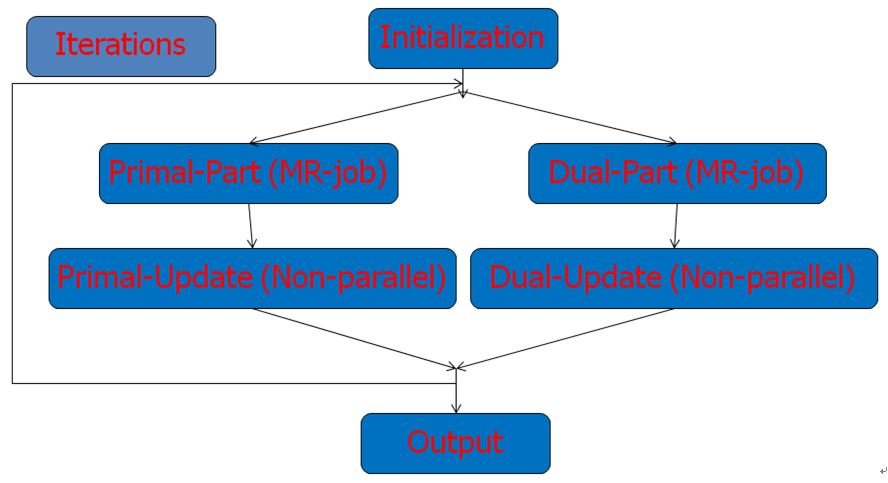
\includegraphics[height=3.0cm,width=6.5cm]{img/framework.png}\vspace{-0.3cm}
\caption{Parallel implementation flow chart for PSUBPLR-MR}\label{fig:frame}\vspace{-0.5cm}
\end{figure}
%

For the parallelization period in the \textit{primal mapreduce job}, we take advantage of the MapReduce design that takes in every data instance.
Instead of the fashion in the sequential algorithm that we only sample one data instance in the primal update step, we compute gradients from ``almost" all data instances and make the weighted average value according to vector $\bp$ as the output gradient for update.
The details of this algorithm design is shown in Procedure Primal-Map and Procedure Primal-Reduce.
Here, we employ a randomization strategy when we compute those ``almost" all gradients.
From line 7 to line 8 in Procedure Primal-Map, all data instances are computed if $r=0$.
As the expectation value for $\bp_t(i_t)$ is $\frac{1}{n}$, we normally set $r$ to range from 0 to 1.
For the parallelization period in the \textit{dual mapreduce job}, we actually implement an embarrassingly parallel operation.
It simply computes an individual value for each data instance in a parallel mode. It does not even need a reduce session.

There are also three more things that need to be handled here.
First is the parameter passing issue. It is critical to choose an efficient way to pass the updated parameters between iterations and even between different MapReduce jobs. Considering the philosophy of the design of Hadoop, the natural thing to do is to pass parameters by file, the same way to pass all the data. We use a single file to pass all parameters each time when a job starts or finishes separately. Although such an operation is insufficiently efficient, it is the feasible way to support large datasets.

The second issue is the small changes that we make to cater for the $\ell_2$-penalty and $\ell_1$-penalty. The changes are only made in Procedure Primal-Update. It affects little for the implementation, and the extension is just the same as that in Algorithm~1. To make the framework brief and standard, we omit the explanation here.

The datasets are generally sparse when data dimensionally is high. This characteristic makes us focus on dealing with data sparsity issue when writing code. Instead of naively writing the simple code in data intensive situations, we only store pairs of \textit{index} and \textit{value} in a data vector. Then all computations are changed accordingly.
This sparse format brings us great efficiency improvement, and all results in Section~\ref{sec:experiment} are obtained from the code for sparsity.

\subsection{Parallel Sublinear algorithms in Spark}
The algorithm to solve sublinear learning for penalized logistic regression in Spark is shown below.
In the pseudo-code of Algorithm 3, the procedure for Primal-Update and the procedure for Dual-Map are the same as those in Algorithm PSUBPLR-MR.
    \begin{table}[ht]
	\begin{tabular}{l}
    \hline\noalign{\smallskip}
	\textbf{Algorithm 3}: PSUBPLR-SPARK \\
	\noalign{\smallskip}
	\hline
	\noalign{\smallskip}
    1:  ~Input parameters: $\varepsilon, \nu~or~\gamma, X, Y, n, d$ \\
    2:	~Initialize parameters: $T, \eta, {\mathbf{u}}_{0}, {\bw}_{1}, {\mathbf{\bq}}_{1}, {b}_{1}$\\
    3:  ~points $\leftarrow$ spark.textFile(inputfile).map(parsePoint()).cache() \\
    4:  ~Iterations: $t=1 \sim T$ \\
    5:  ~\tspace gradient $\leftarrow$ points.map($(\frac{1}{1+e^{-y((\bw_t^T \textbf{x})+b)}}-1) * y * \bp [index]$) \\
        ~~~\tspace\tspace\tspace\tspace\tspace .reduce(sum()) \\
    6:  ~\tspace ($\bw_{t+1}, b_{t+1}$)$\leftarrow$Primal-Update($\bw_t, b_t$) \\
    7:  ~\tspace Choose $j_t \leftarrow j$ with probability ${{\bw}_{t+1}\lj}^{2}/{\|{\bw}_{t+1}\|_2}^{2} $ \\
    8:  ~\tspace pAdjust $\leftarrow$ points.map(MW-Update()).reduce(copy()) \\
    9:  ~\tspace $\bp_{t+1}\leftarrow$Dual-Update($\bp_t$)  \\
    10: \textbf{Output}($\bw, b$) \\
    \hline
    \end{tabular}
	\end{table}

This parallel design is very similar to that of Algorithm PSUBPLR-MR.
The most important difference is the \textit{cache()} operation in line 3.
To make it work in Spark, we follow the rule to construct an RDD for each data instance.
Also to cater for data sparsity, the design is that every data value correspond to its individual \textit{index}. And the \textit{index} is also involved in the computation along with the value.
We omit the changes for $\ell_2$-penalty and $\ell_1$-penalty here to make the algorithm easier to be understood.

In parallel mode, the primal update contains the update of $\bw_t$, which takes $O(n)$ time.
The dual update contains the $\ell_2$-sampling process for the choice of $j_t$ in $O(d)$ time, and the update of $\bp$ in $O(1)$ time.
Altogether, each iteration takes $O(n+d)$ time.
Compared to the analysis of sequential algorithm, parallelization does not necessarily change computational complexity.
Theoretically, parallel sublinear algorithm can be two times faster than the sequential version as the time for both update procedures in each iteraion is reduced to $O(1)$.
Moreover, by starting two separate MapReduce jobs in one iteration simultaneously, the running time can be reduced to $O(max\{n,d\})$.

\subsection{Parallel Gradient Descent in Spark}
The parallel gradient descent method to solve LR in Spark is shown below.
    \begin{table}[ht]
	\begin{tabular}{l}
    \hline\noalign{\smallskip}
	\textbf{Algorithm 4}: PGDPLR-SPARK \\
	\noalign{\smallskip}
	\hline
	\noalign{\smallskip}
    1:  Input parameters: $\varepsilon, \nu~or~\gamma, X, Y, n, d$ \\
    2:	Initialize parameters: $T, \eta, {\mathbf{u}}_{0}, {\bw}_{1}, {\mathbf{\bq}}_{1}, {b}_{1}$\\
    3:  points $\leftarrow$ spark.textFile(inputfile).map(parsePoint()).cache() \\
    4:  Iterations: $t=1 \sim T$ \\
    5:  \tspace gradient $\leftarrow$ points.map($(\frac{1}{1+e^{-y((\bw_t^T \textbf{x})+b)}}-1)*y$) \\
        ~~\tspace\tspace\tspace\tspace\tspace .reduce(sum()) \\
    6:  \tspace $\bw_{t+1} = \bw_t - gradient * \textbf{x}$ \\
    7:  \tspace $b = b - gradient$ \\
    8:  \textbf{Output}($\bw, b$) \\
    \hline
    \end{tabular}
	\end{table}

In the pseudo-code of Algorithm 4, it is implemented in an embarrassingly parallel mode.
We can take in all data at the same iteration and just compute the gradient in a MapReduce fashion.
As for the \textit{cache()} operation and RDD design for data sparsity, it is the same with Algorithm PSUBPLR-SPARK.

\subsection{Online Stochastic Gradient Descent in Mahout}
Though SGD is an inherently sequential algorithm, it is blazingly fast. Thus Mahout's implementation can handle training sets of tens of millions of examples.
The SGD system in Mahout is an online learning algorithm, implying that we can learn models in an incremental fashion and perform testing when the system runs.
In addition, we can halt training when a model reaches a target level of performance.
Because the SGD algorithms need feature vectors of fixed length and it is very costly to build a dictionary ahead of time, most SGD applications use an encoding system to derive hashed feature vectors. We can create a \textit{RandomAccessSparseVector}, and then use various feature encoders to progressively add features to this vector.

In our implementation, we use \textit{RandomAccessSparseVector} for data sparsity and the function call by \textit{OnlineLogisticRegression} to train the LR classifier.
We also perform cross validation. However, to keep consistent with other methods, we write our own code to do cross validation.
	
\section{Experimental Setup} \label{sec:setup}
This section presents the details of the dataset information, cluster information, and the test programs of our experiments.

\subsection{Dataset Information}
We choose five open datasets to run all six test programs. Details are shown in Table~\ref{tab:table1}.	
Different from the simulated \textbf{2d} dataset, the other four datasets are all sparse.
We split each dataset into the training set and the testing set. We randomly repeat such split 20 times and our analysis is based on the average performance of 20 repetitions. In Table~\ref{tab:table1}, \textit{Density} is computed as
\[
Density(Dataset)~=~\frac{\#~of~Nonzeros}{\#~of~all~entries},
\]
which stems from~\cite{sarwar2001item}.
\textit{Balance} describes the binary distribution of labels.
We compute it as following:
\[
Balance(Dataset)~=~\frac{\#~of~Positive~Instances}{\#~of~Negative~Instances}.
\]
\begin{table*}%[h]
\centering
\caption{Datasets}\label{tab:table1}\vspace{-0.3cm}
\begin{tabular}{|c|c|c|c|c|c|c|c|}
\hline
    Name           & Dimension & \# of instances & Density  & \# of nonzero values & Balance & \# of training & \# of testing\\
\hline
    2d             & 2             & 200            & 1.0                      & 400          & 1.000 & --- & --- \\
\hline
    20NewsGroup    & 16428         & 1988           & $7.384\times10^{-3}$     & 238511          & 1.006 & 1800 & 188\\
\hline
    Gisette        & 5000          & 7000           & 0.12998                  & 4549319          & 1.000 & 6000 & 1000\\
\hline
    ECUESpam       & 100249        & 10687          & $2.563\times10^{-3}$     & 2746159          & 5.882 & 9000 & 1687\\
\hline
    URL-Reputation & 3231961       & 2376130        & $3.608\times10^{-5}$     & 277058644          & 0.500 & 2356130 & 20000\\
\hline
\end{tabular}\vspace{-0.3cm}
\end{table*}
These five datasets are carefully selected with an incremental trend in size.
The simulated \textbf{2d} dataset represents toy data situations and serves for the initial test of correctness of classifiers.
The \textbf{20NewsGroup} dataset is best-known for the test of LR model, which has a balanced distribution between positive and negative data instances. It also shows the application towards topic classification.
The \textbf{Gisette} dataset~\cite{guyon2004result} is relatively larger, and feature vectors are less sparse.
The \textbf{ECUESpam} dataset~\cite{DelanyKBS05} is selected due to its imbalanced distribution between positive and negative data instances. It has a higher data dimensionality than the \textbf{Gisette} dataset. However, because of data sparsity, it has fewer nonzero values involved in the computation.
Finally, the \textbf{URL-Reputation} dataset~\cite{ma2009identifying} contains millions of data instances and features. The raw data are stored in the svmlight format, which has the volume of more than 2GB. It can be seen as a representative of massive datasets in the sense that it exceeds the scalability of Liblinear, which will be shown below.

\subsection{Cluster Information}
The cluster that we implement on has the configurations shown in Table~\ref{tab:table2}.
\begin{table}[h]
\centering
\caption{Cluster Information}\label{tab:table2}\vspace{-0.3cm}
\begin{tabular}{|c|c|}
\hline
    CPU Model & Intel Xeon E5-1410: 2.80GHz \\
\hline
    Number of node & 6 \\
\hline
    Number of CPU per node & 4 Cores, 8 Threads \\
\hline
    RAM per node & 16G \\
\hline
    Disk per node & 4T HDD\\
\hline
    Interconnection Method & Gigabyte Ethernet  \\
\hline
\end{tabular}
\end{table}
This kind of cluster configuration is now more and more common in research labs. Hence our results reported in the following can have a real impact in the research community.

\subsection{Test Programs}
There are all together 6 test programs for comparison.
Online stochastic gradient descent method is run on Mahout in a sequential mode.
Liblinear~\cite{fan2008liblinear} is also a baseline test program we choose. It is sequential and outperforms many other programs for LR on a single machine.
SLLR performs the sequential sublinear algorithm on a single machine.
PSUBPLR-MR performs the parallel sublinear algorithm on Hadoop on cluster.
PGDPLR-SPARK is the test program for the parallel gradient descent run on Spark.
PSUBPLR-SPARK implements the parallel sublinear algorithm run on Spark.

\section{Experimental Results} \label{sec:experiment}
In this section, we conduct empirical analysis on experimental results.
We show four things: 1) accuracy, 2) efficiency, 3) scalability and 4) robustness.

\subsection{Results on Precision} \label{sec:precision}
The results of six test programs achieved on five datasets are shown in Table~\ref{tab:table3}.
%
\begin{table}[h]
\centering
\caption{Accuracy Results. The meanings of abbreviations are as follows: 20-N-G, 20 News Group; URL-R, URL-Reputation.}\label{tab:table3}\vspace{-0.3cm}
\begin{tabular}{|c|c|c|c|c|}
\hline
           & 20-N-G & Gisette & ECUESpam & URL-R \\
\hline
Mahout     & 71.3\% & 91.5\% & 85.2\% & 91.5\% \\
\hline
Liblinear  & \textbf{92.0\%} & \textbf{97.4\%} & \textbf{97.1\%} & --- \\
\hline
SLLR       & 91.5\% & 94.8\% & 92.3\% & 94.2\% \\
\hline
PSUBPLR-MR & 90.5\% & 94.6\ & 91.7\% & 93.8\% \\
\hline
PGDPLR-SPARK & \textbf{92.0\%} & 97.0\% & 93.7\% & \textbf{96.0\%} \\
\hline
PSUBPLR-SPARK & 90.5\% & 95.8\% & 91.7\% & 94.0\% \\
\hline
\end{tabular}
\end{table}
%
These are the averaged results of cross validation.
In Figures~\ref{fig:accuracy} (a)-(d), we show the test error as a function of iteration number on each dataset for all six test programs.
Note that Liblinear cannot be implemented with the full \textbf{URL-Reputation} dataset on our machine due to memory limit.
This proves the scalability issue of Liblinear.
In the tests, Liblinear can handle $33.3\%$ of the whole data volume at most, with the test accuracy of $96.2\%$ and the running time of 519s.
%
\begin{figure*}[tb]
\begin{center}
\begin{tabular}{cccc}
   %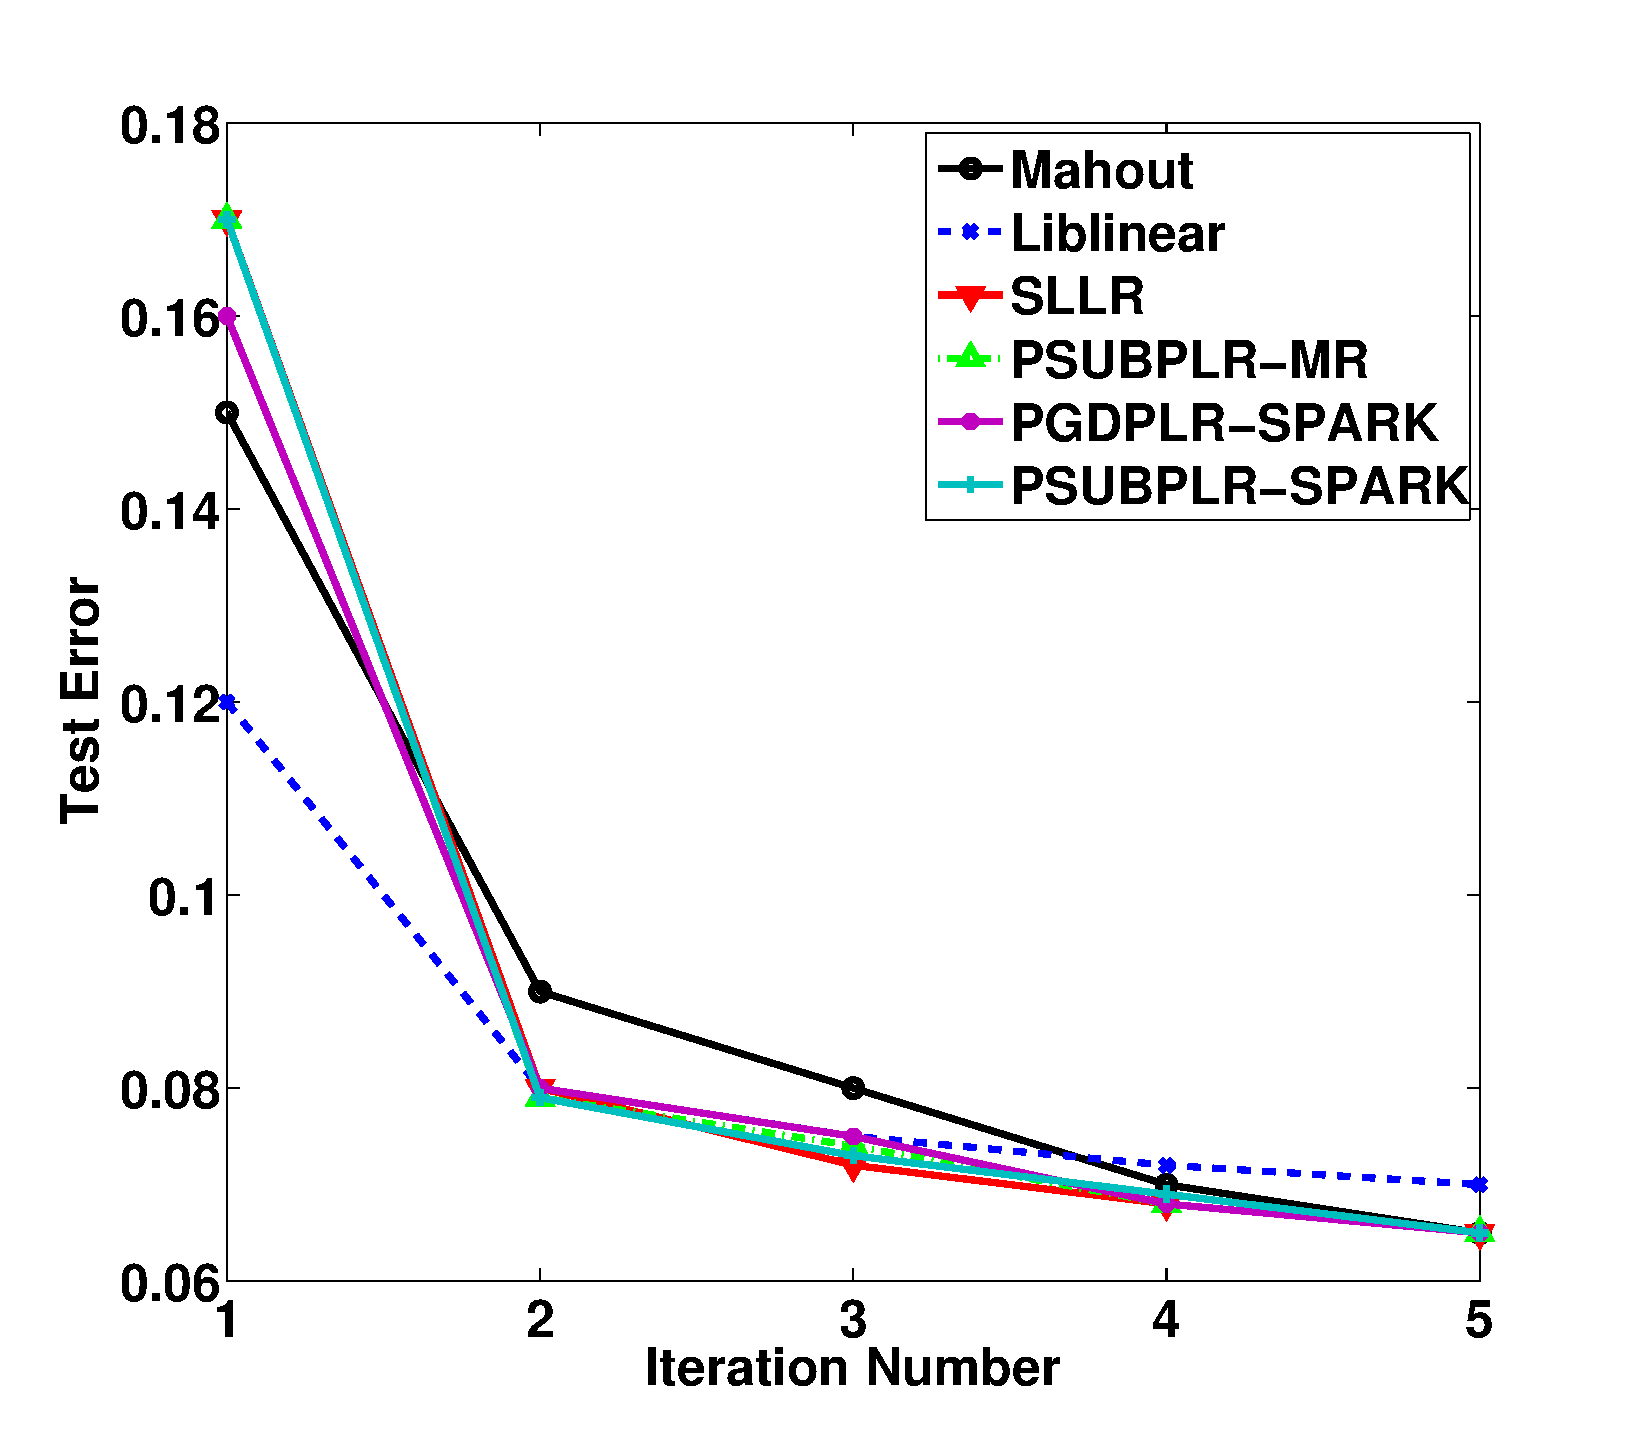
\includegraphics[height=4.5cm,width=5cm]{img/2d_accuracy_iteration.eps}&
   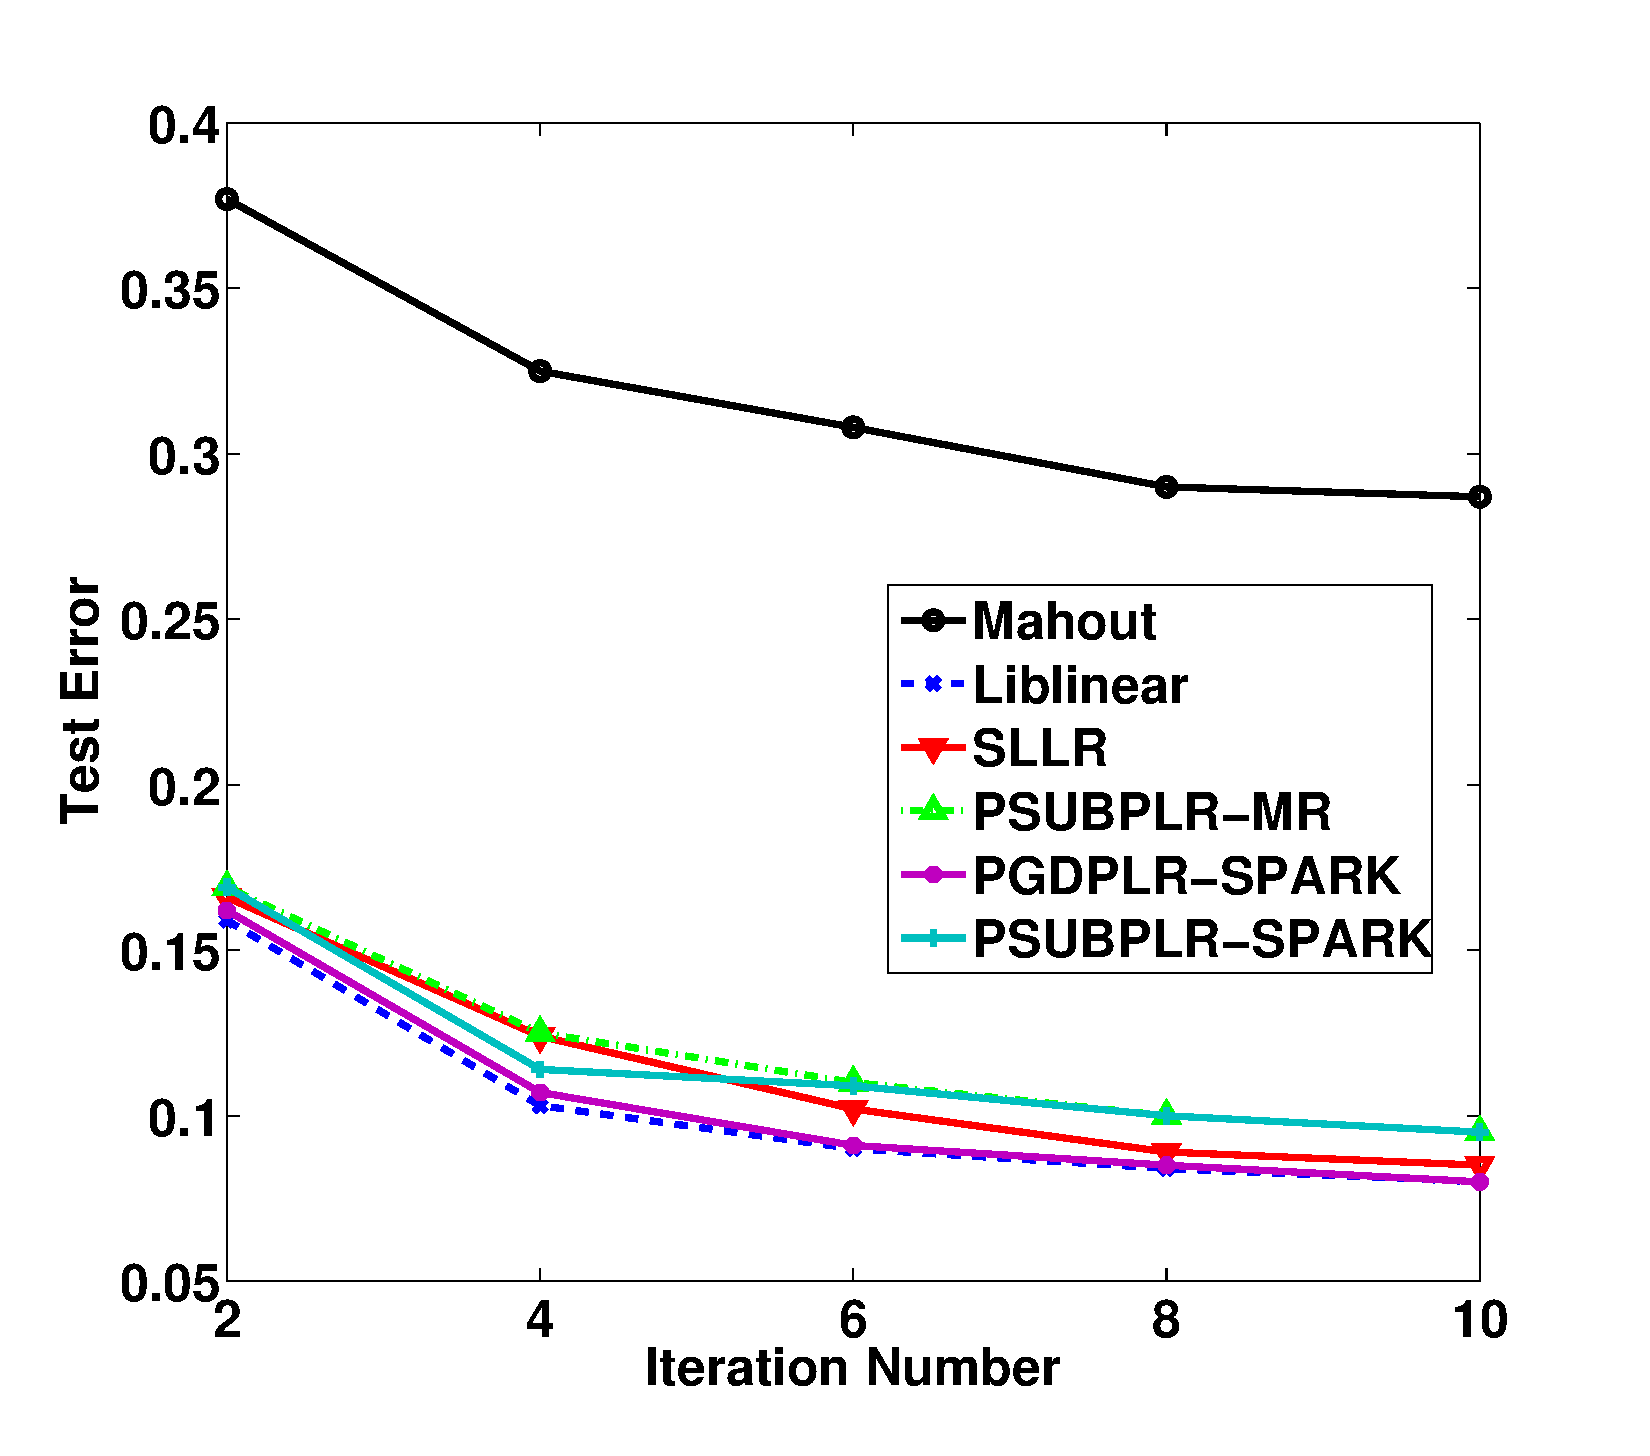
\includegraphics[height=4.cm,width=4.5cm]{img/20NewsGroup_accuracy_iteration.eps}&
   \hspace{-0.6cm}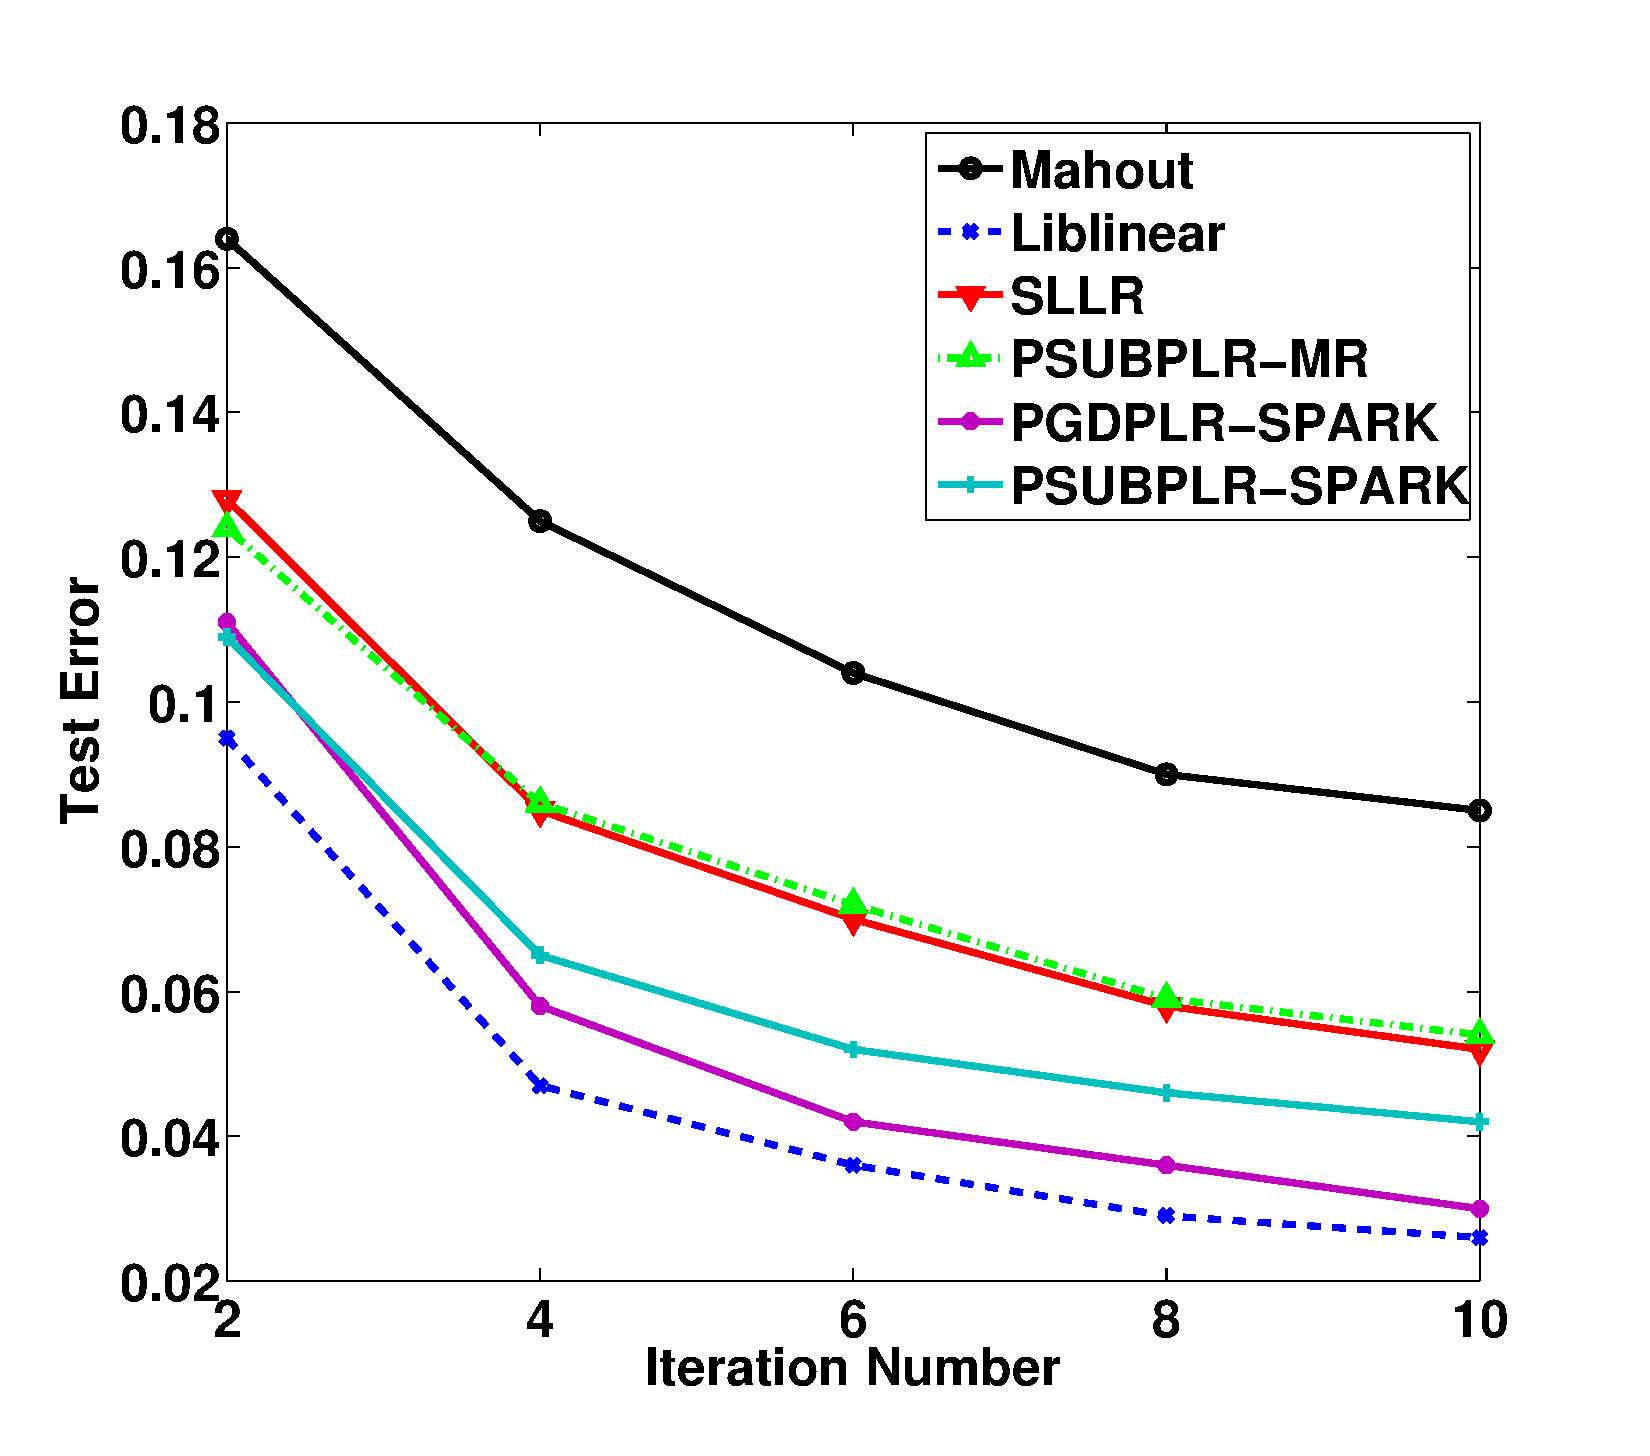
\includegraphics[height=4.cm,width=4.5cm]{img/Gisette_accuracy_iteration.eps}&
   \hspace{-0.6cm}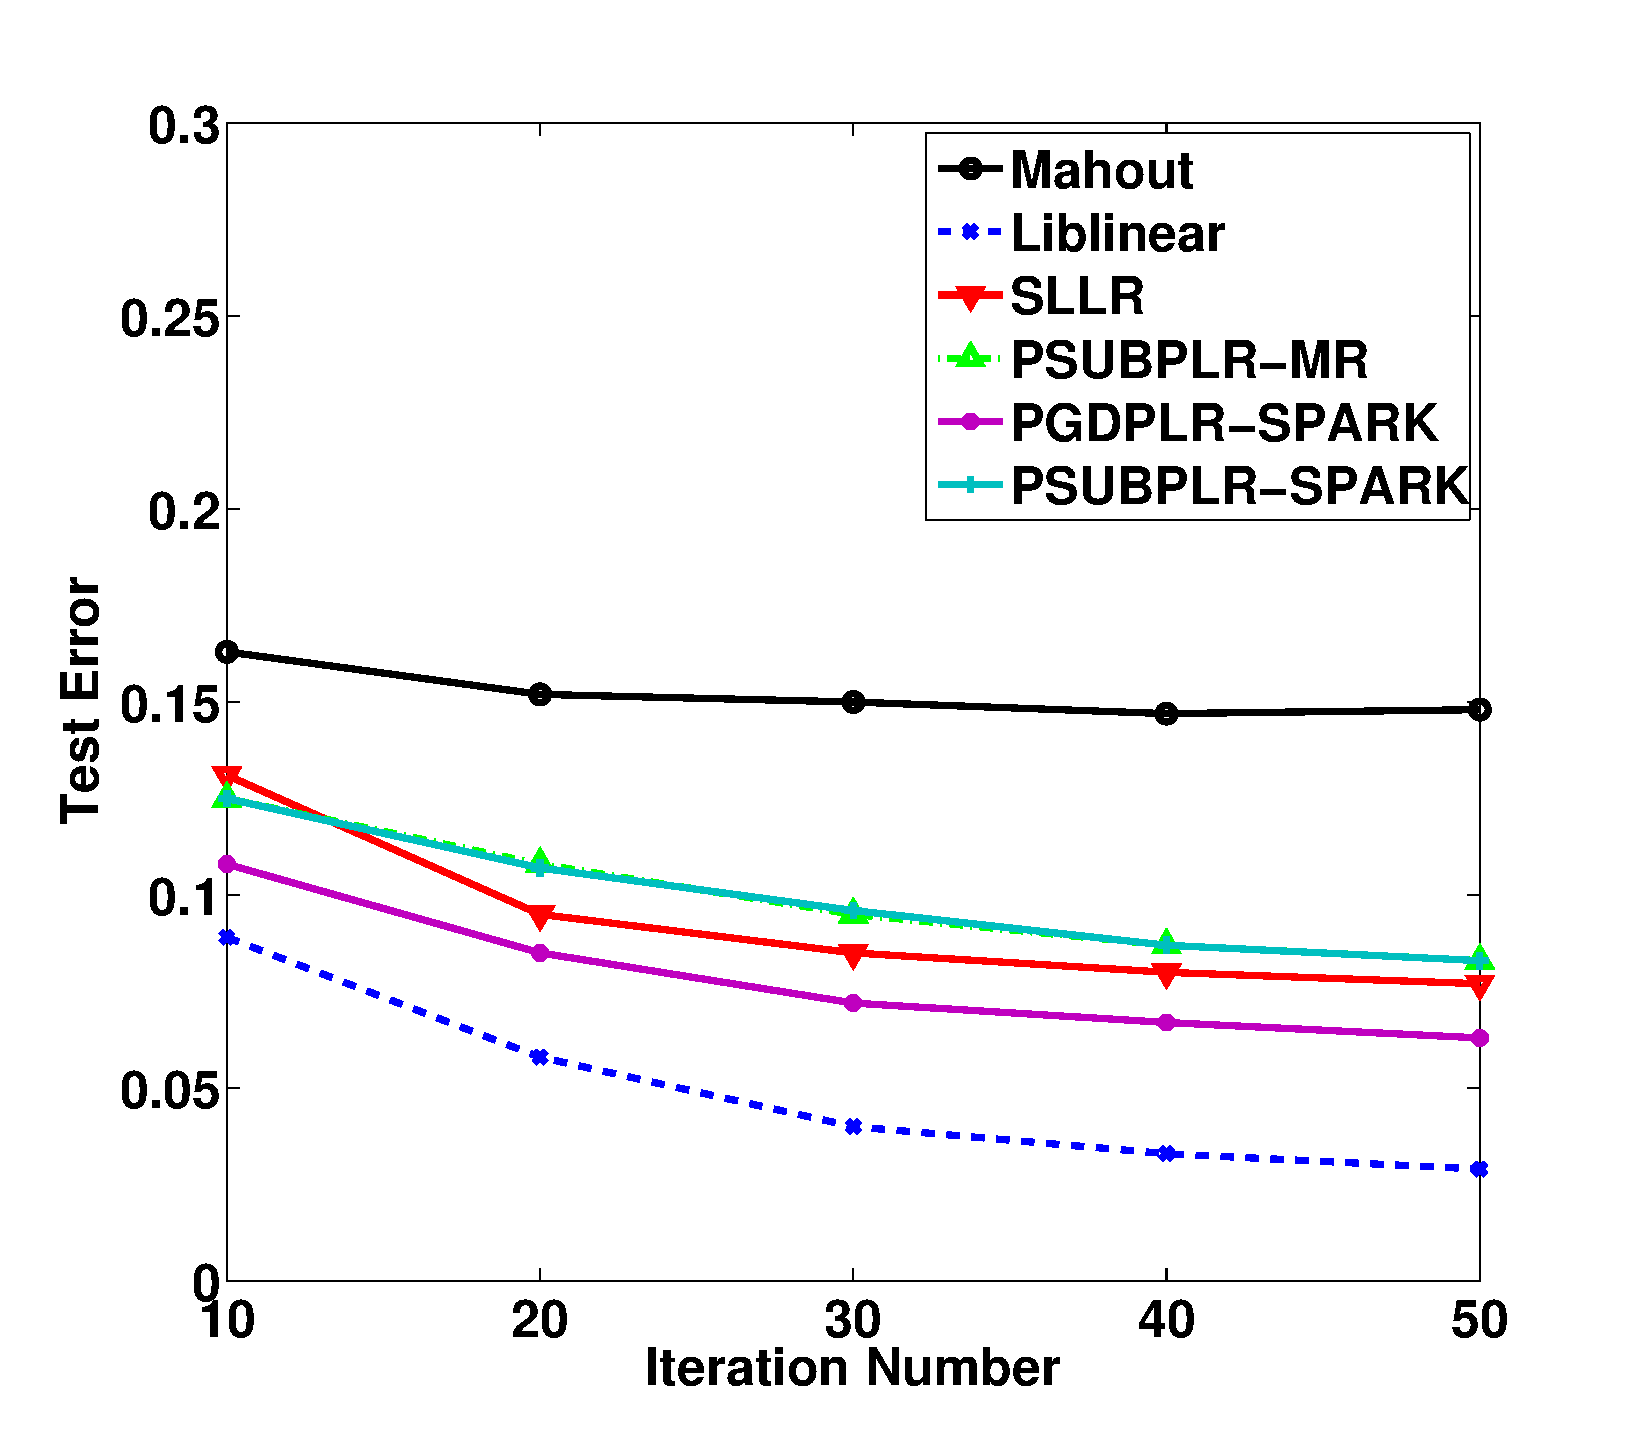
\includegraphics[height=4.cm,width=4.5cm]{img/ECUESpam_accuracy_iteration.eps}&
   \hspace{-0.6cm}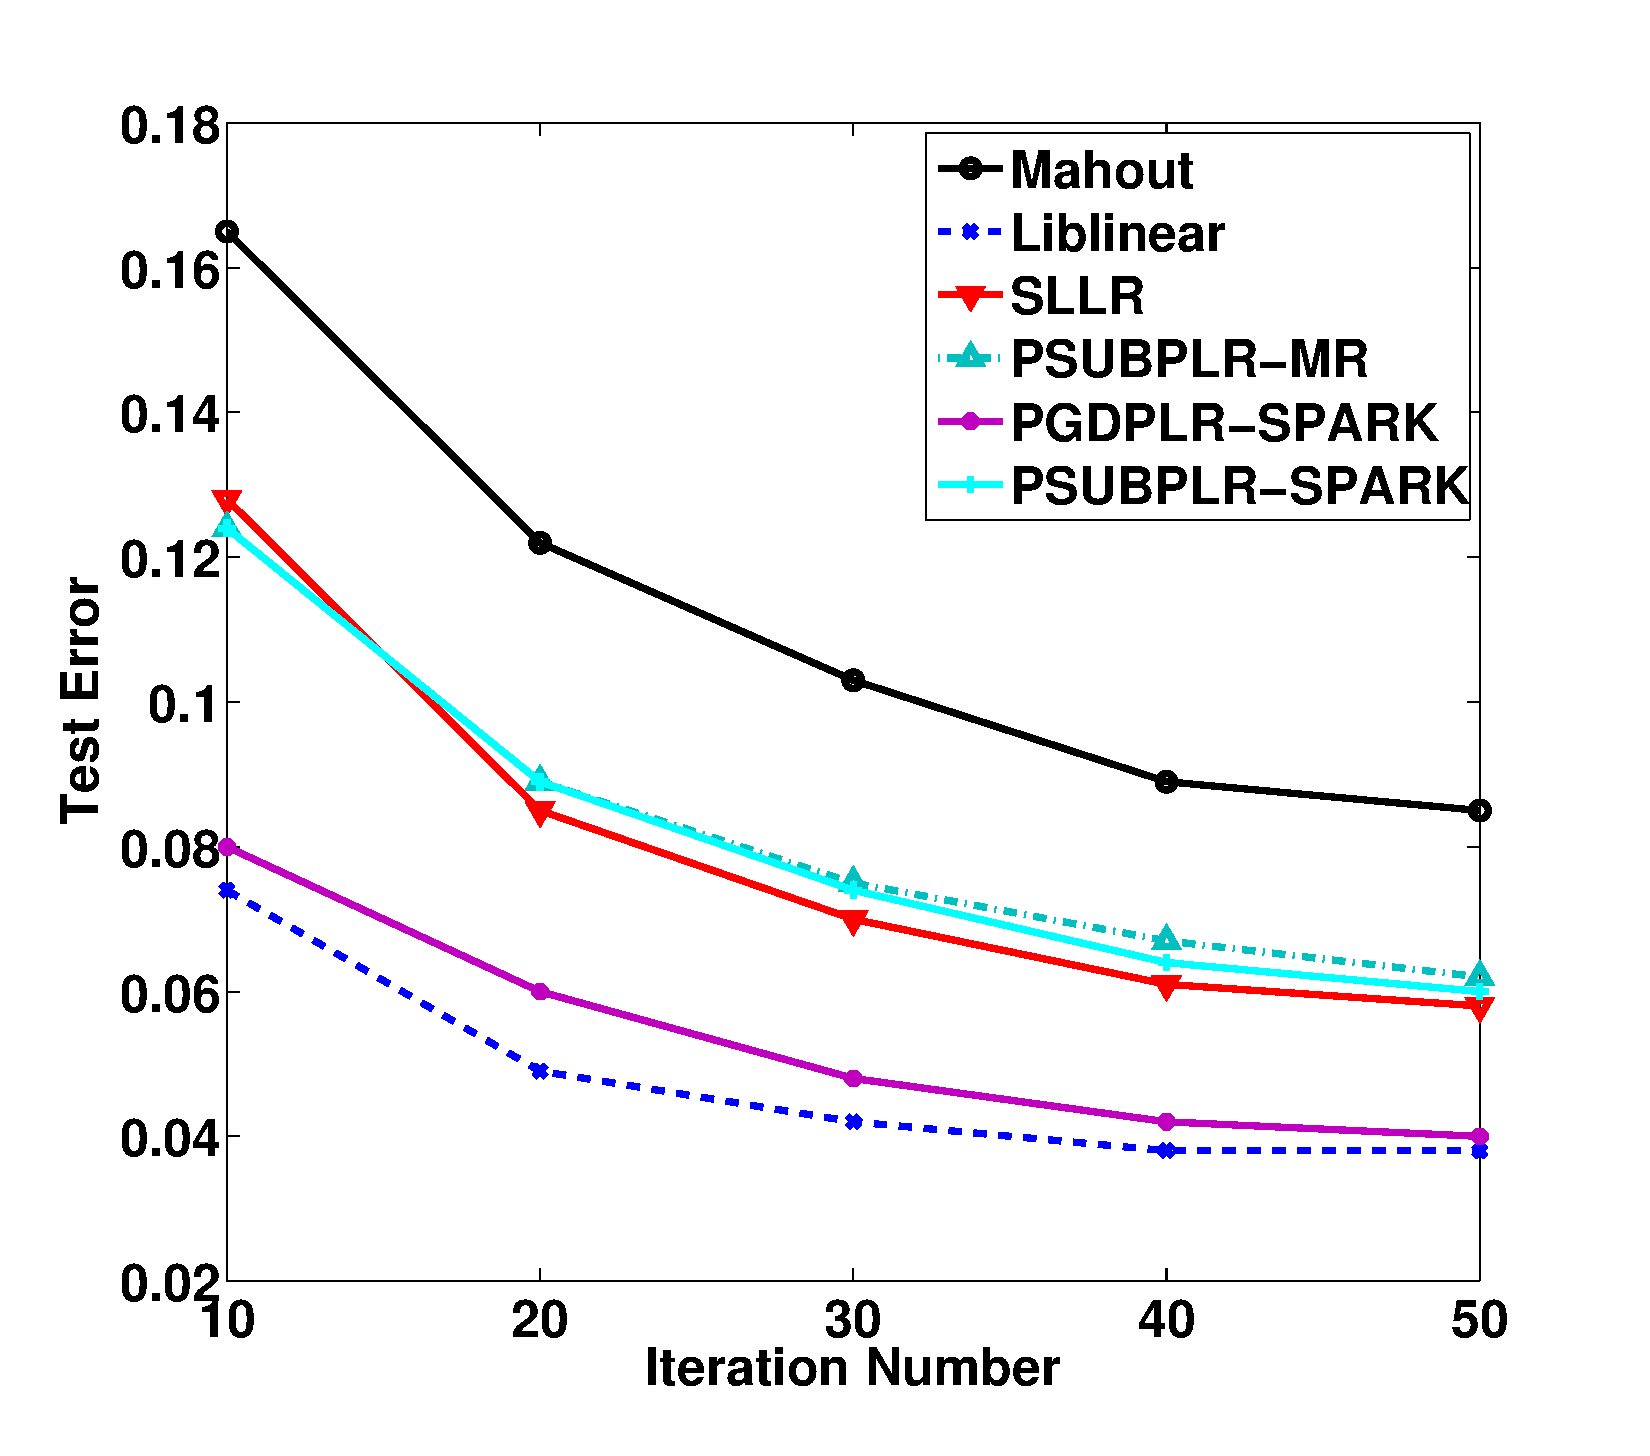
\includegraphics[height=4.cm,width=4.5cm]{img/URL-Reputation_accuracy_iteration.eps}\\
   (a) \textbf{20NewsGroup}. & \hspace{-0.3cm}(b) \textbf{Gisette}. & \hspace{-0.3cm}(c) \textbf{ECUESpam}. & \hspace{-0.3cm}(d) \textbf{URL-Reputation}.\\
   \end{tabular}
\end{center}\vspace{-0.3cm}
   \caption{Test error, as a function of iteration number.}\vspace{-0.5cm}
\label{fig:accuracy}
\end{figure*}

\subsection{Results on Running Time} \label{sec:time}

The running time of six test programs used on five datasets is shown in Table~\ref{tab:table4}.
These are the averaged results corresponding to the accuracies we achieved in Table~\ref{tab:table3}.
%
\begin{table}[h]
\centering
\caption{Running Time. The meanings of abbreviations are as follows: 20-N-G, 20 News Group; URL-R, URL-Reputation.}\label{tab:table4}\vspace{-0.3cm}
\begin{tabular}{|c|c|c|c|c|c|}
\hline
           & 20-N-G & Gisette & ECUESpam & URL-R \\
\hline
Mahout     & 9.83s & 131.8s & 96s & 10100s \\
\hline
Liblinear  & \textbf{0.79s} & \textbf{2.4s} & \textbf{13s} & --- \\
\hline
SLLR       & 20.05s & 130.5s & 1028s & 3248s \\
\hline
PSUBPLR-MR & 1360.85s & 3687.9s & 11478s & 16098s \\
\hline
PGDPLR-SPARK & 10.52s & 99.2s & 924s & 3615s \\
\hline
PSUBPLR-SPARK & 8.57s & 89.1s & 796s & \textbf{2918s} \\
\hline
\end{tabular}
\end{table}

In another way, we show the running time results in Fig.~\ref{fig:08} for comparison.
\begin{figure}[tb]
\center 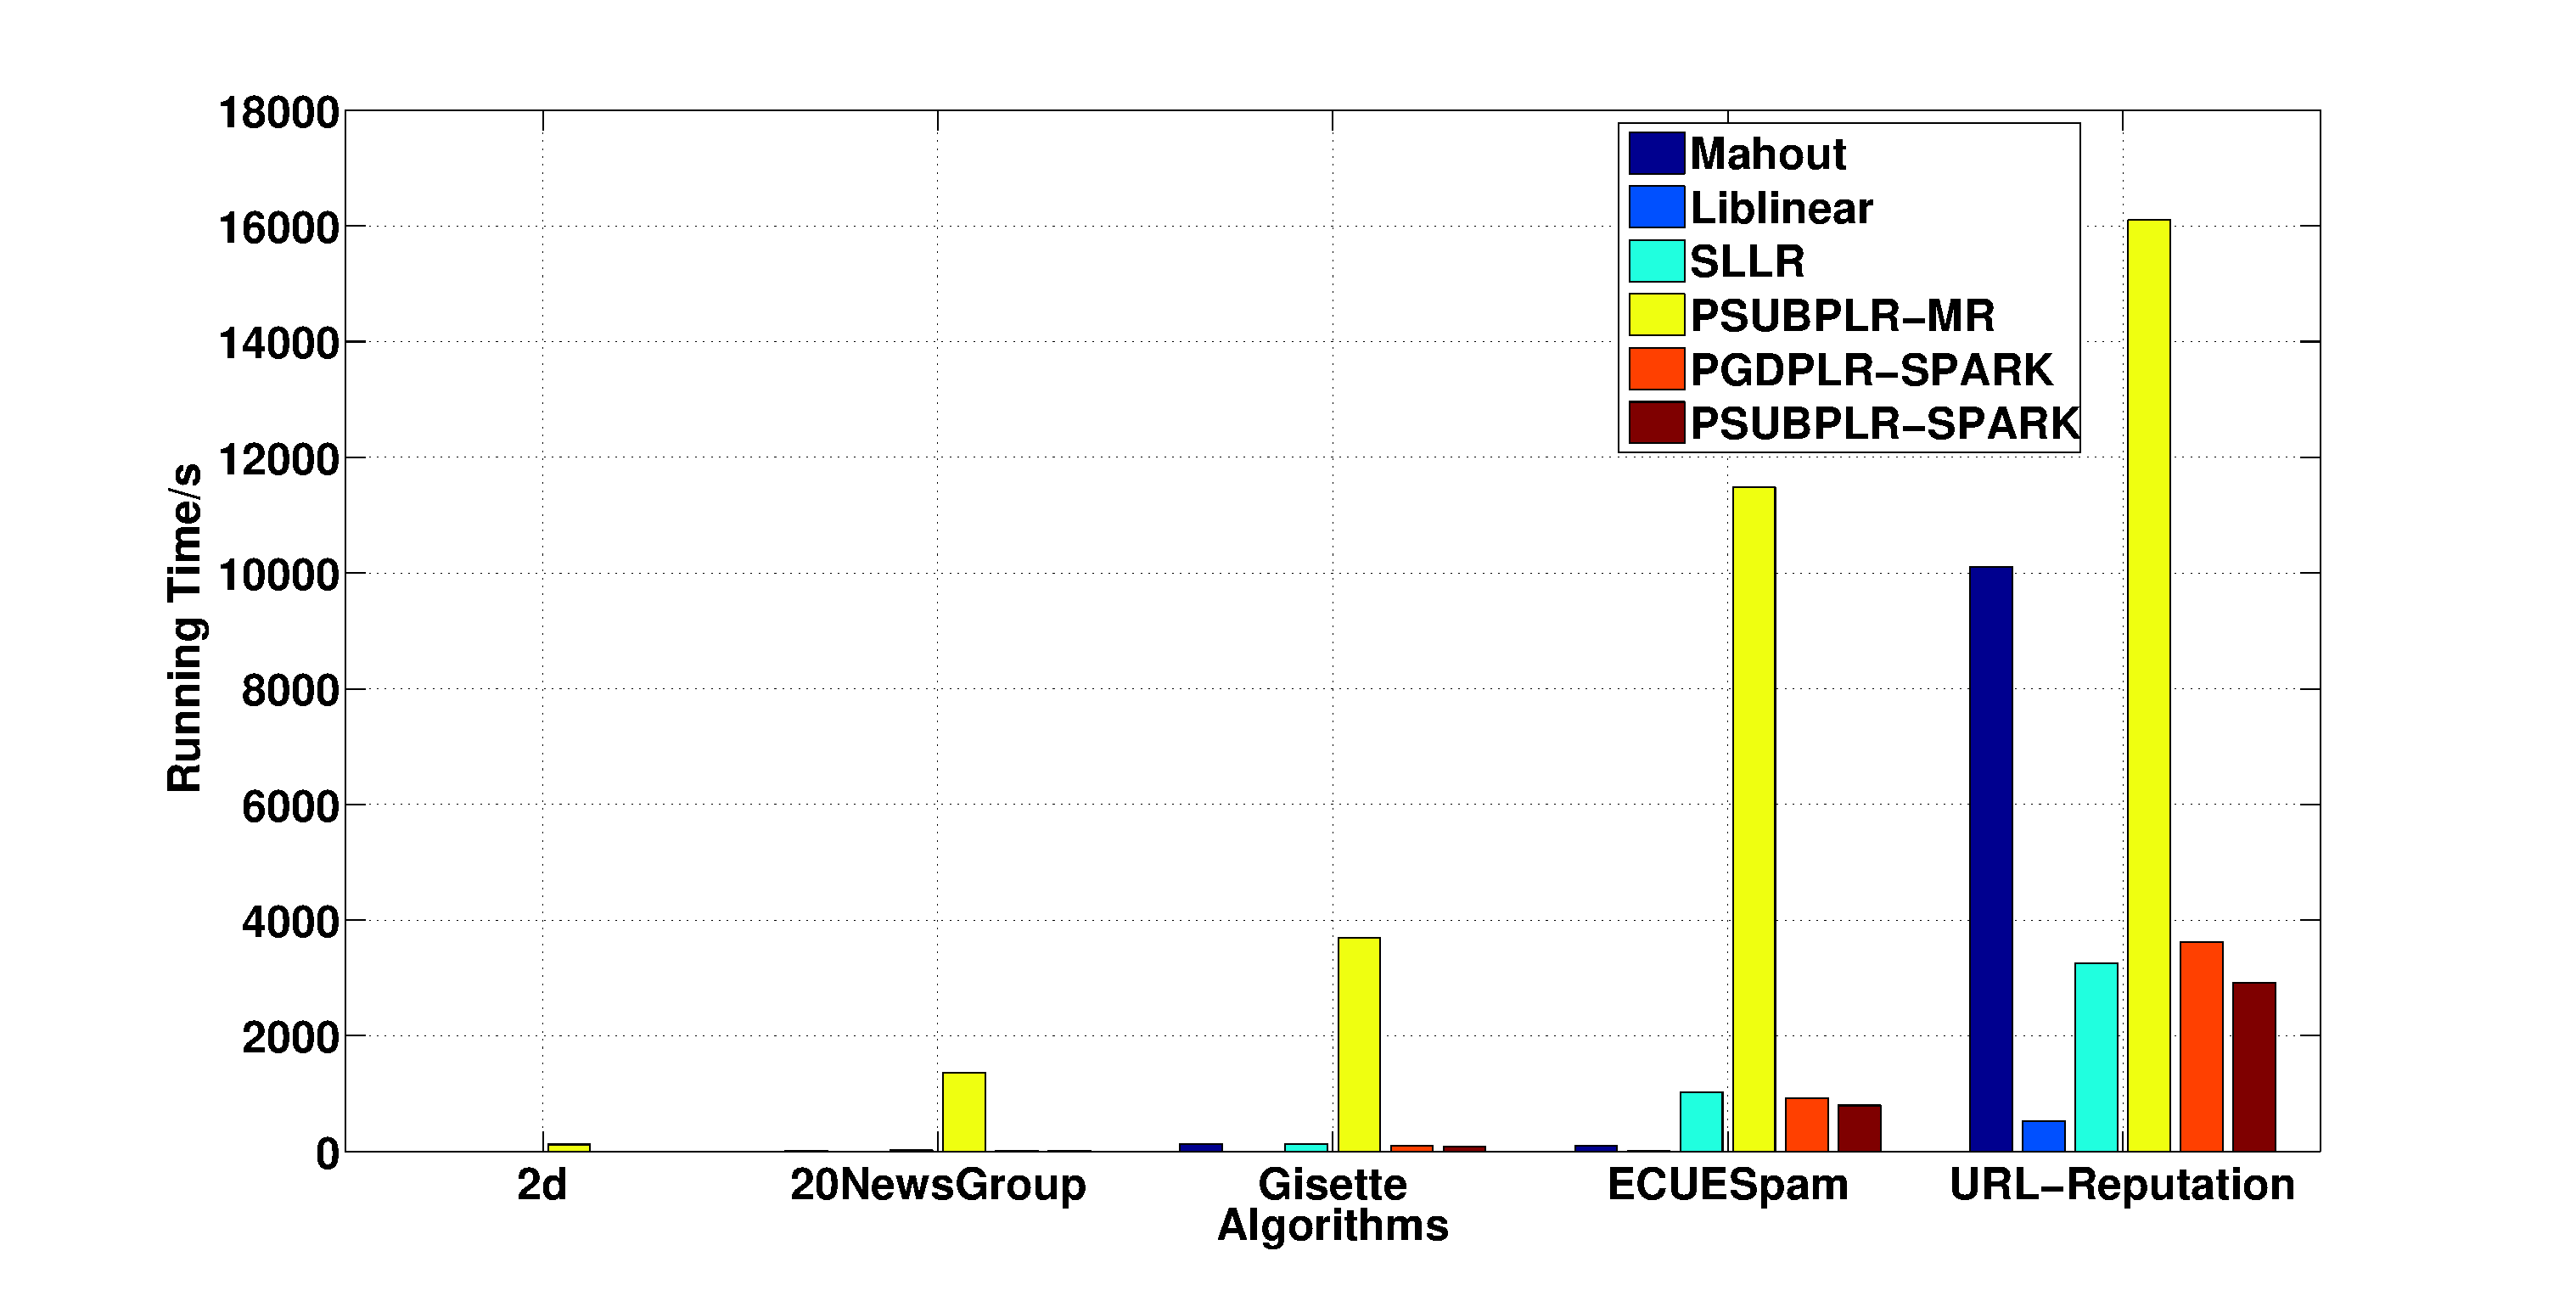
\includegraphics[height=4.5cm,width=9cm]{img/all_time.eps}\vspace{-0.3cm}
\caption{Running time.}\label{fig:08}\vspace{-0.5cm}
\end{figure}

From the accuracy results in Section~\ref{sec:precision} and the running time results in Section~\ref{sec:time}.
We can come up with following conclusions.

1) Liblinear performs best. It fully utilizes memory and the single machine implementation does not require any communication between machines.
          However, its scalability is limited by the memory size of the single machine that it runs on, which prevents its use for massive datasets.
          Nevertheless, if the dataset can be fully loaded into the memory of a single machine, this efficient and direct sequential way of implementation is still recommended.

2) Mahout's precision is not good, especially for those datasets in which positive and negative instances are imbalanced.
          However, it is a representative example of sequential algorithm that can train massive data in acceptable time.
          When we monitor its memory when running, it is much lower than Liblinear. This is the advantage brought by both online algorithm and hashing operations on features.
          Therefore, it provides good scalability guarantee. If you are in the situation of single machine and limited memory, sequential online training like Mahout is recommended.

3) The precision of all sublinear methods is acceptable. The developed parallel sublinear algorithm only has a small drop in precision.

4) Hadoop system has a drawback for running LR optimization methods. Its cluster programming model is based on acyclic data flow from stable storage to stable storage.
          Though it has the benefits of deciding where to run tasks and can automatically recover from failures in runtime, acyclic data flow is inefficient for iterative algorithms.
          All six test programs contain a number of iterations, thus making PSUBPLR-MR performs poorly, even worse than sequential algorithms.
          When we study the details of Hadoop implementation, we find that the MapReduce job starting time in PSUBPLR-MR is about 20s. It consists of task configuration time and parameter passing time.
          This running time overhead is not negligible, especially when dataset is relatively small.
          We also identify that the running of ``Primal-Map" dominates the whole iteration time (more than 66\%). It is the same situation for PSUBPLR-SPARK.

5) Spark employs the ``all-in-memory" strategy, and it constructs RDD on demand. We implement PGDPLR-SPARK and PSUBPLR-SPARK in normal file system instead of HDFS.
          Current results on Spark show that it is much more efficient than Hadoop, and performs better than Mahout.
          In the parallel situation, we recommend Spark to process massive data. Further, we recommend to choose PSUBPLR-SPARK for less running time in exchange for a little bit precision loss.
          As the platform is still under developing process, we expect that our running time results for PGDPLR-SPARK and PSUBPLR-SPARK can still be improved.

6) Another interesting point we would like to raise is about dataset. If we compare \textbf{ECUESpam} dataset and \textbf{GISETTE} dataset.
          The former has higher data dimensionality but more sparse.
          Compare the data point between Figure~\ref{fig:time}(b) and~\ref{fig:time}(c) We can find that algorithms on \textbf{ECUESpam} dataset enjoy less running time per iteration than on \textbf{GISETTE} dataset as \textbf{ECUESpam} has fewer nonzero values involved in the computation.
          However, algorithms on \textbf{ECUESpam} dataset need more iterations than on \textbf{GISETTE} dataset, which is related to higher data dimensionality of \textbf{ECUESpam} dataset. This even causes more running time in total.
          To sum up, to get a general sense of running time for individual dataset, we need to consider both data volume and sparsity.

\subsection{Results on Changing Cluster}
In Figures~\ref{fig:time} (a)-(d), we show the running time as a function of used node number on each dataset for all three parallel test programs.
%
\begin{figure*}[tb]
\begin{center}
\begin{tabular}{cccc}
   %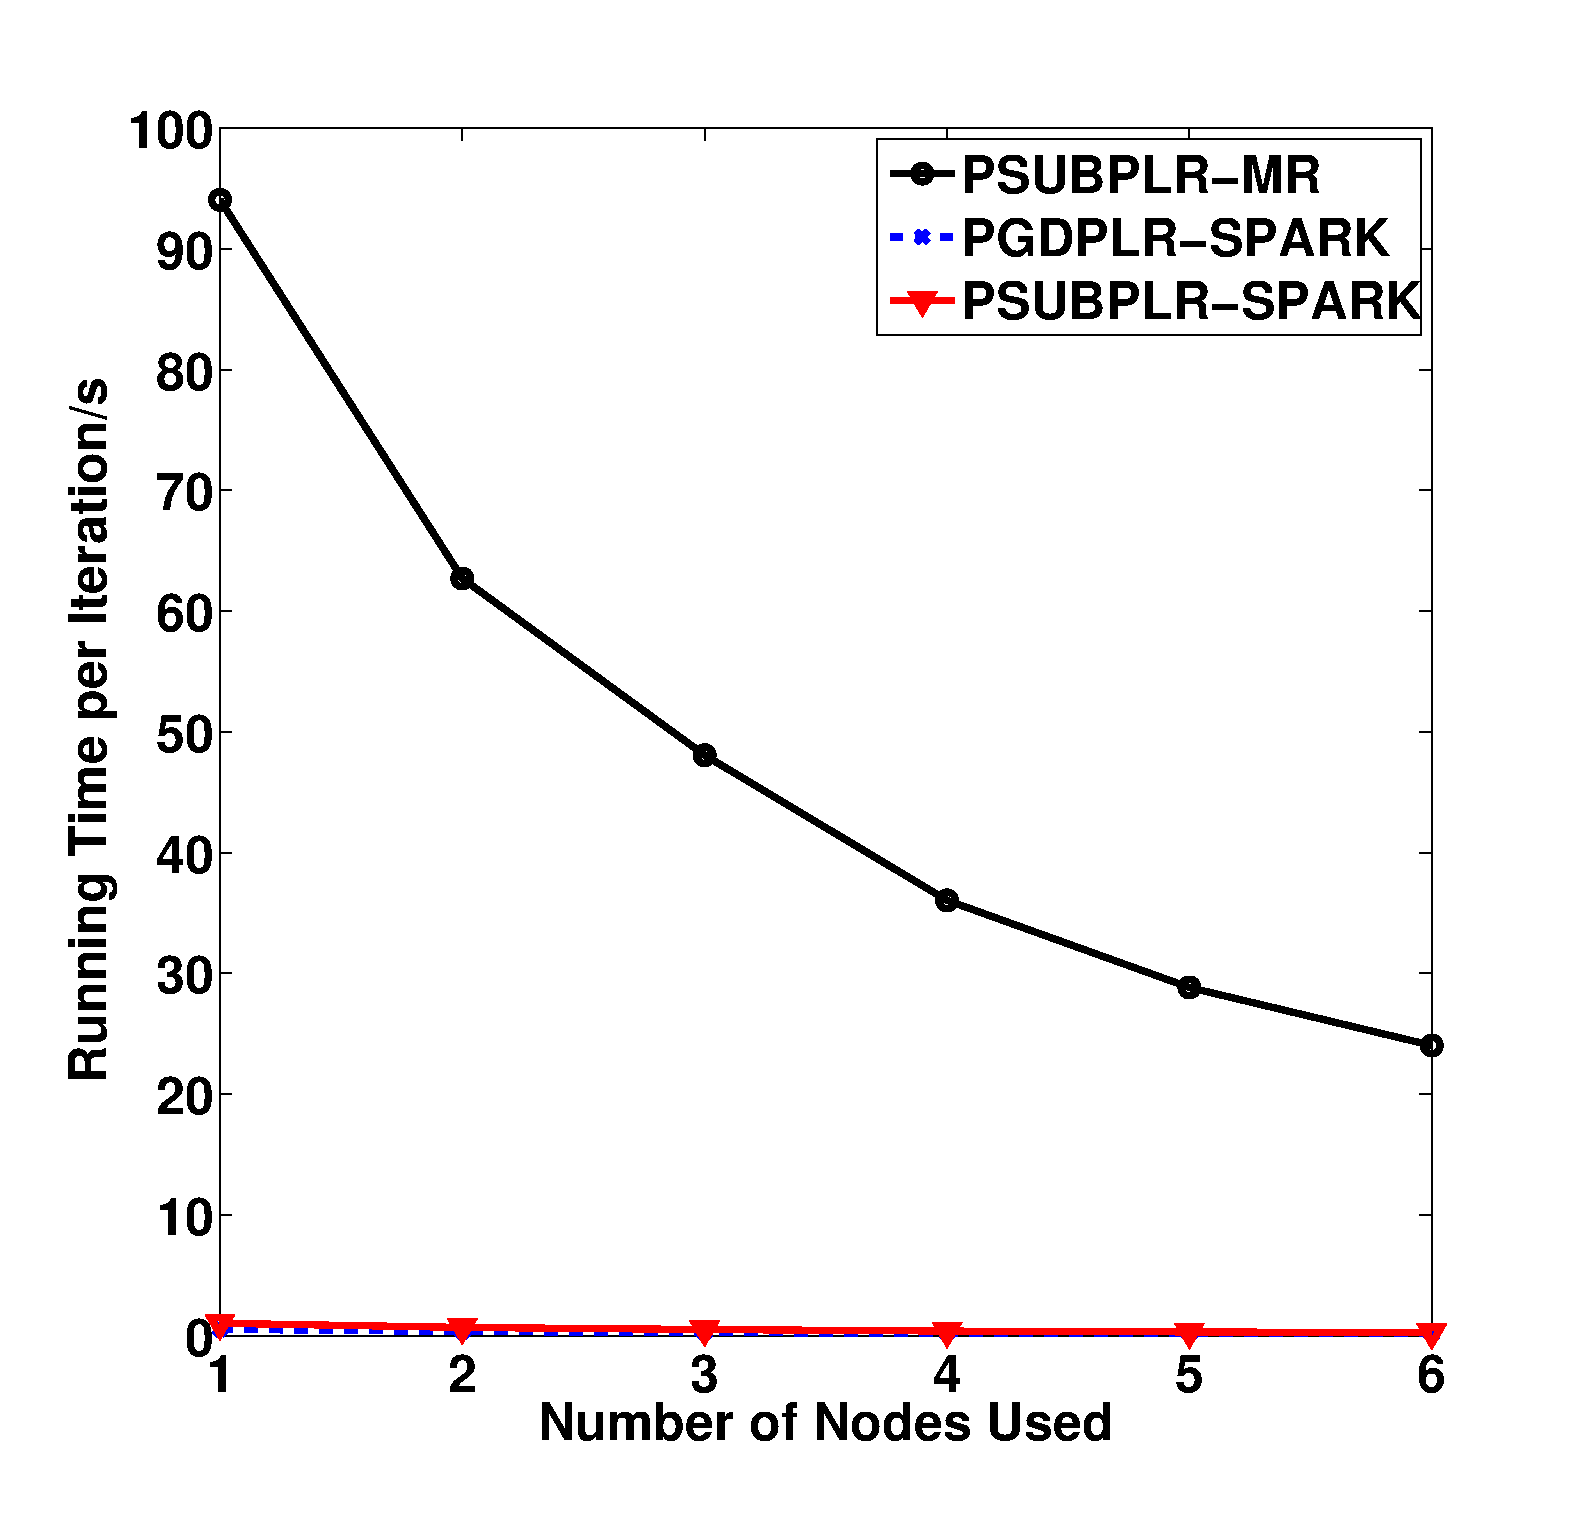
\includegraphics[height=4.5cm,width=5cm]{img/2d_time.eps}&
   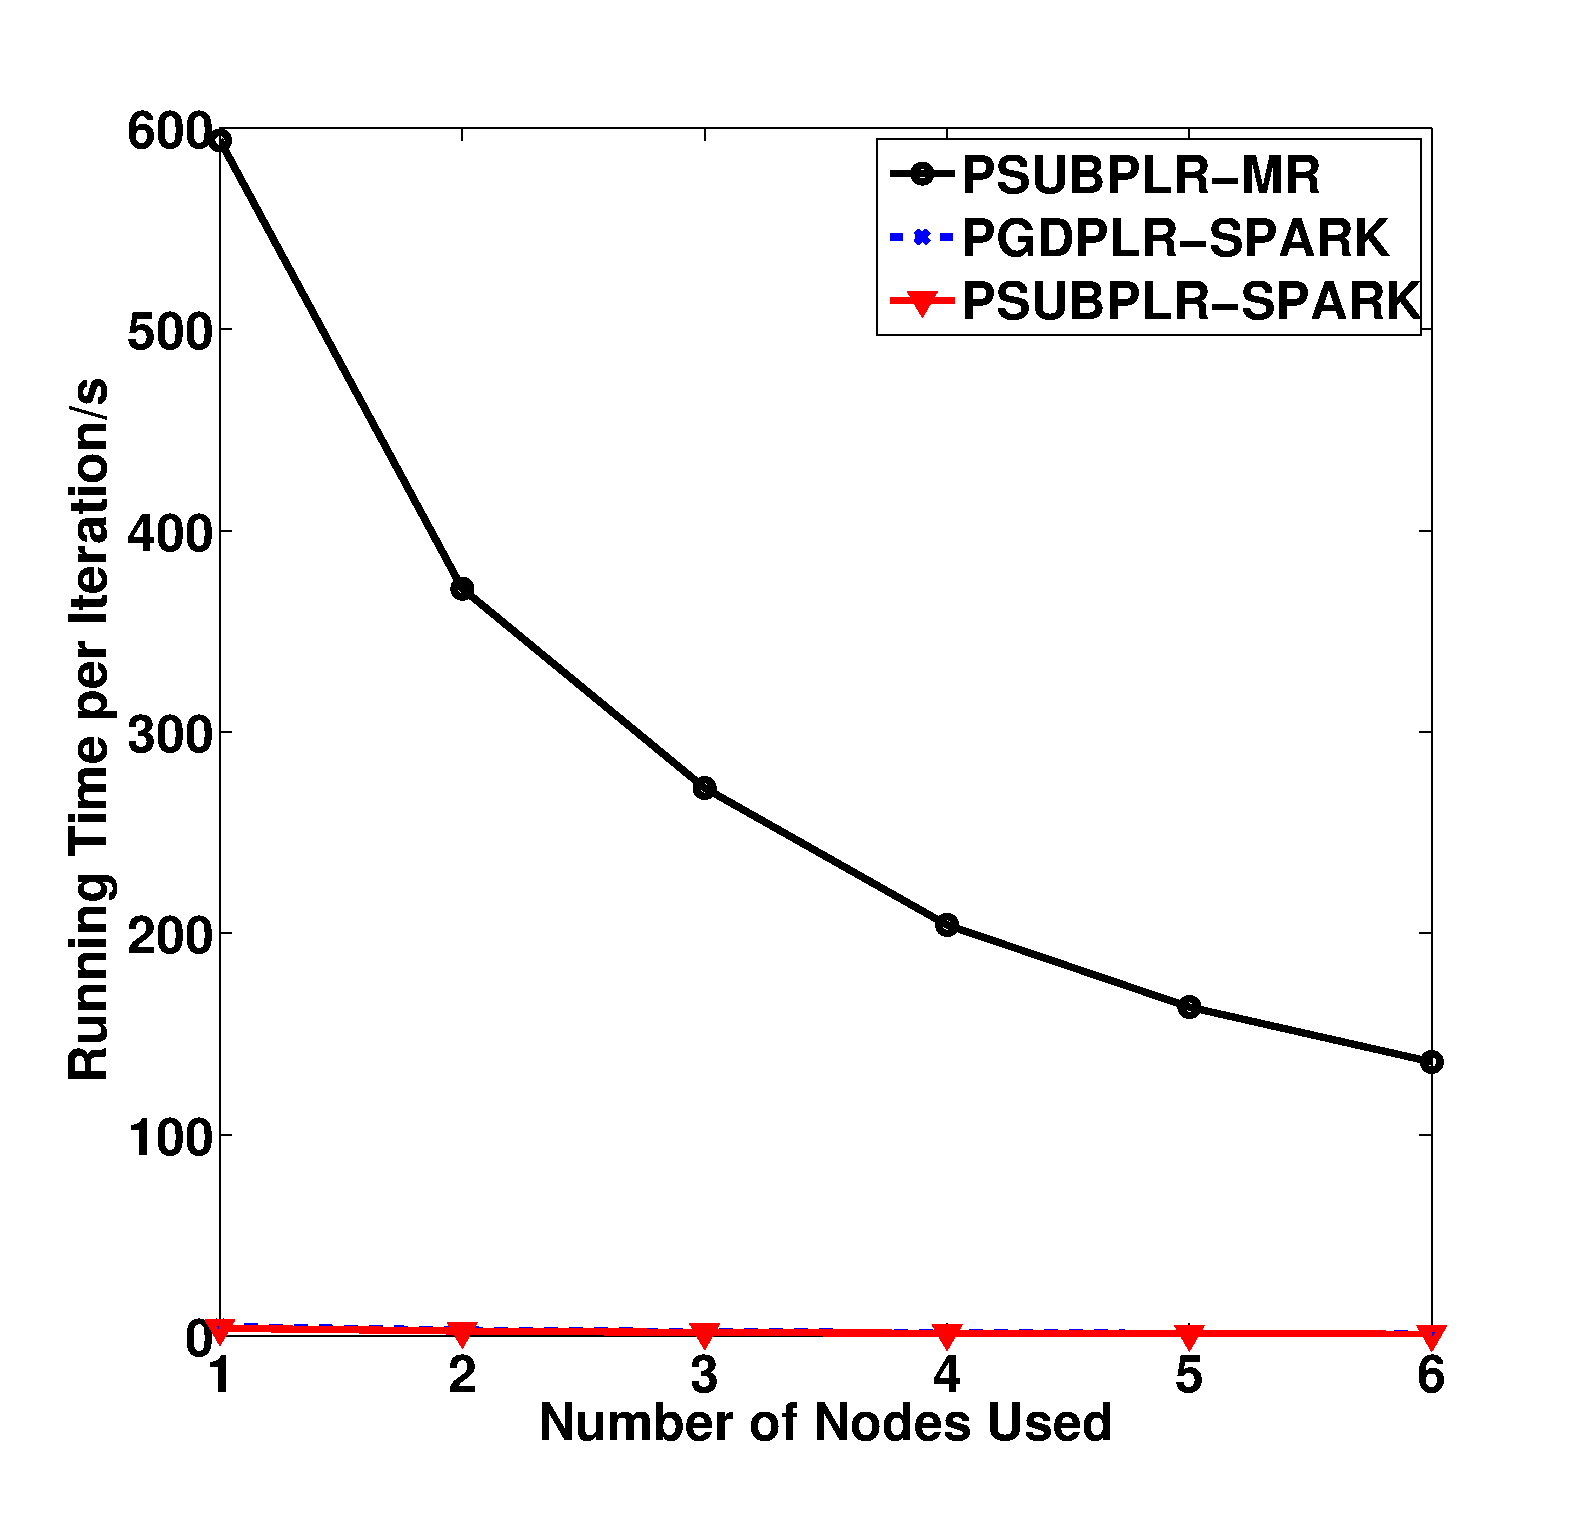
\includegraphics[height=3.9cm,width=4.5cm]{img/20NewsGroup_time.eps}&
   \hspace{-0.6cm}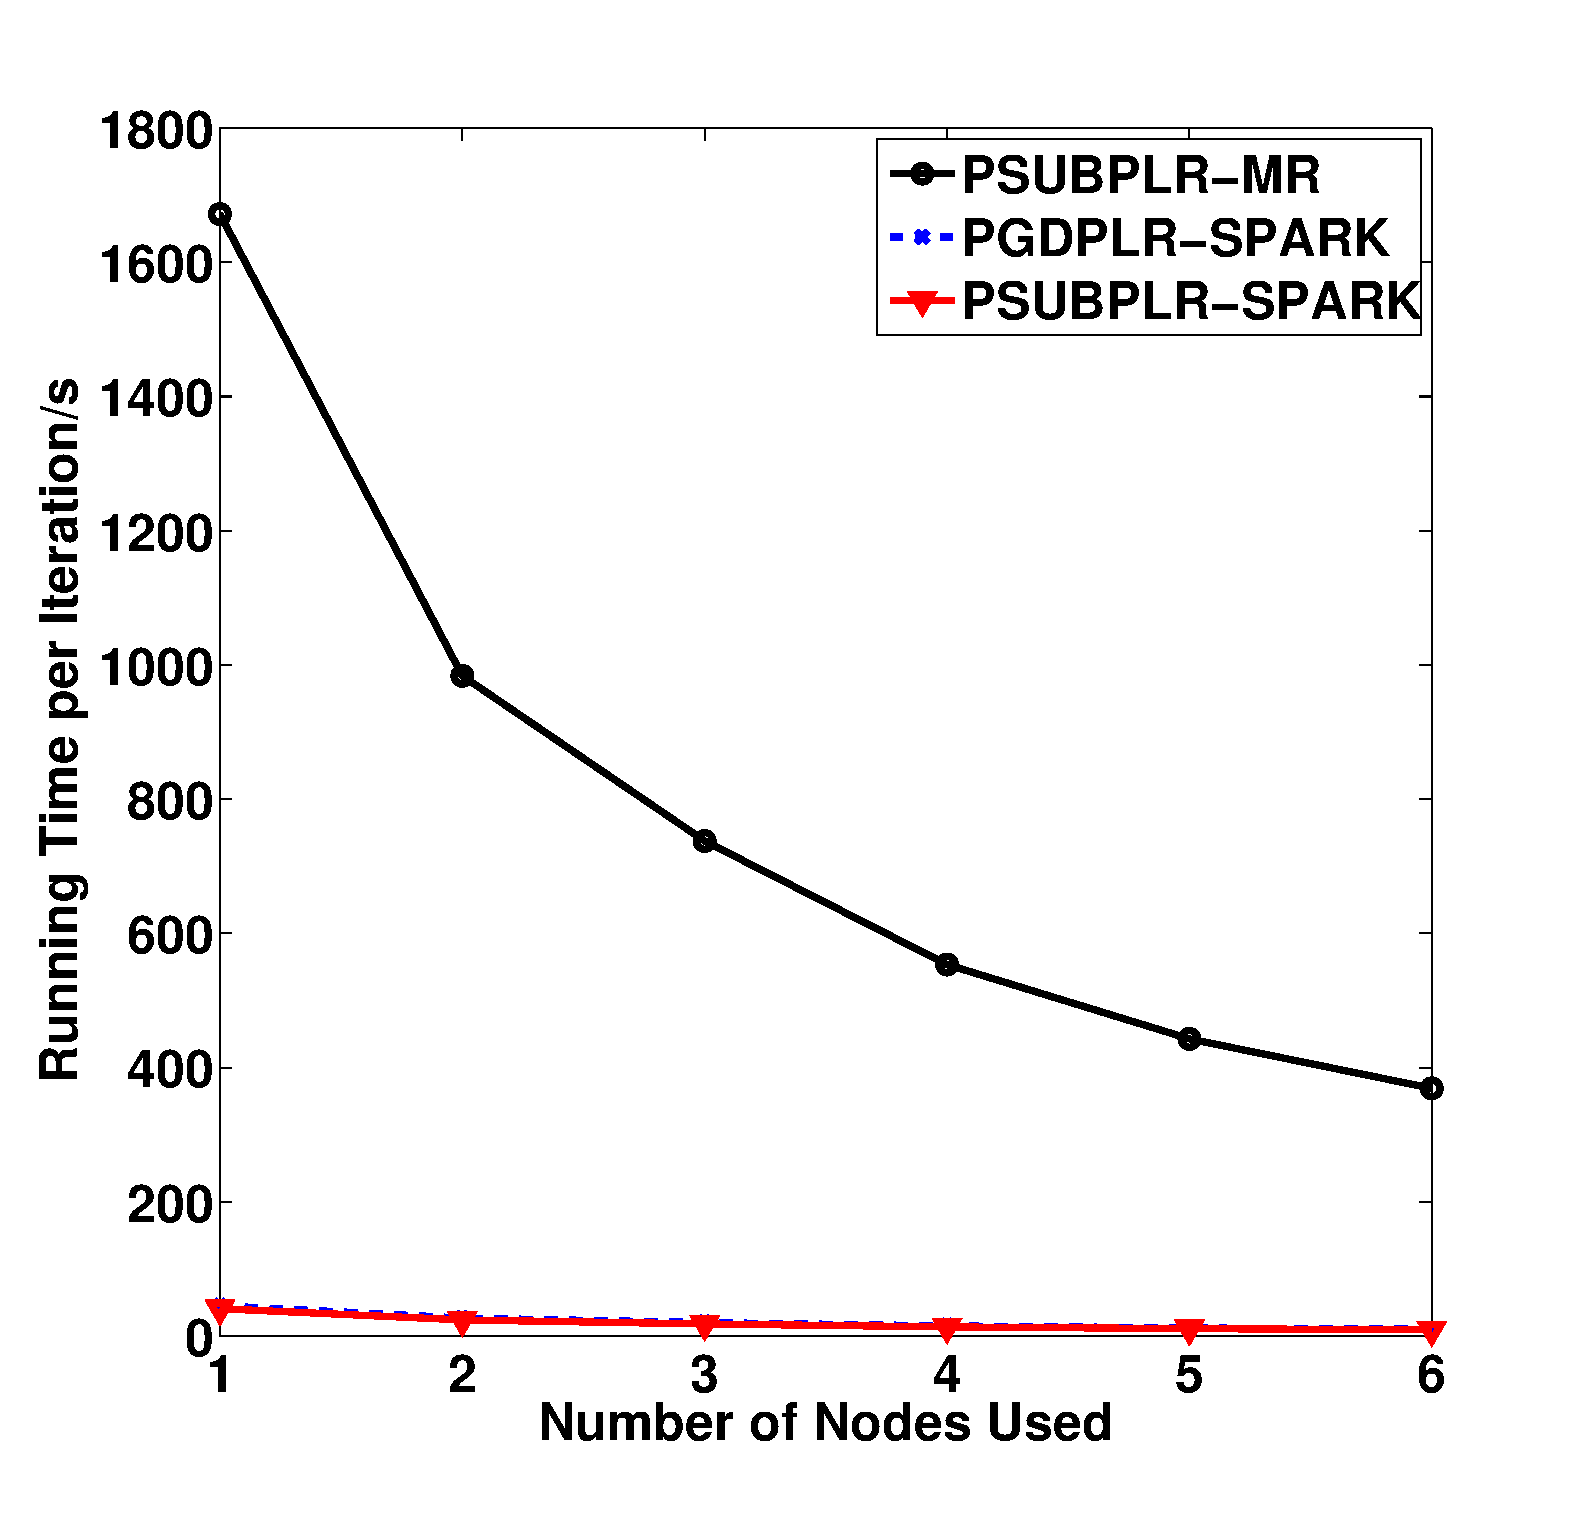
\includegraphics[height=3.9cm,width=4.5cm]{img/Gisette_time.eps}&
   \hspace{-0.6cm}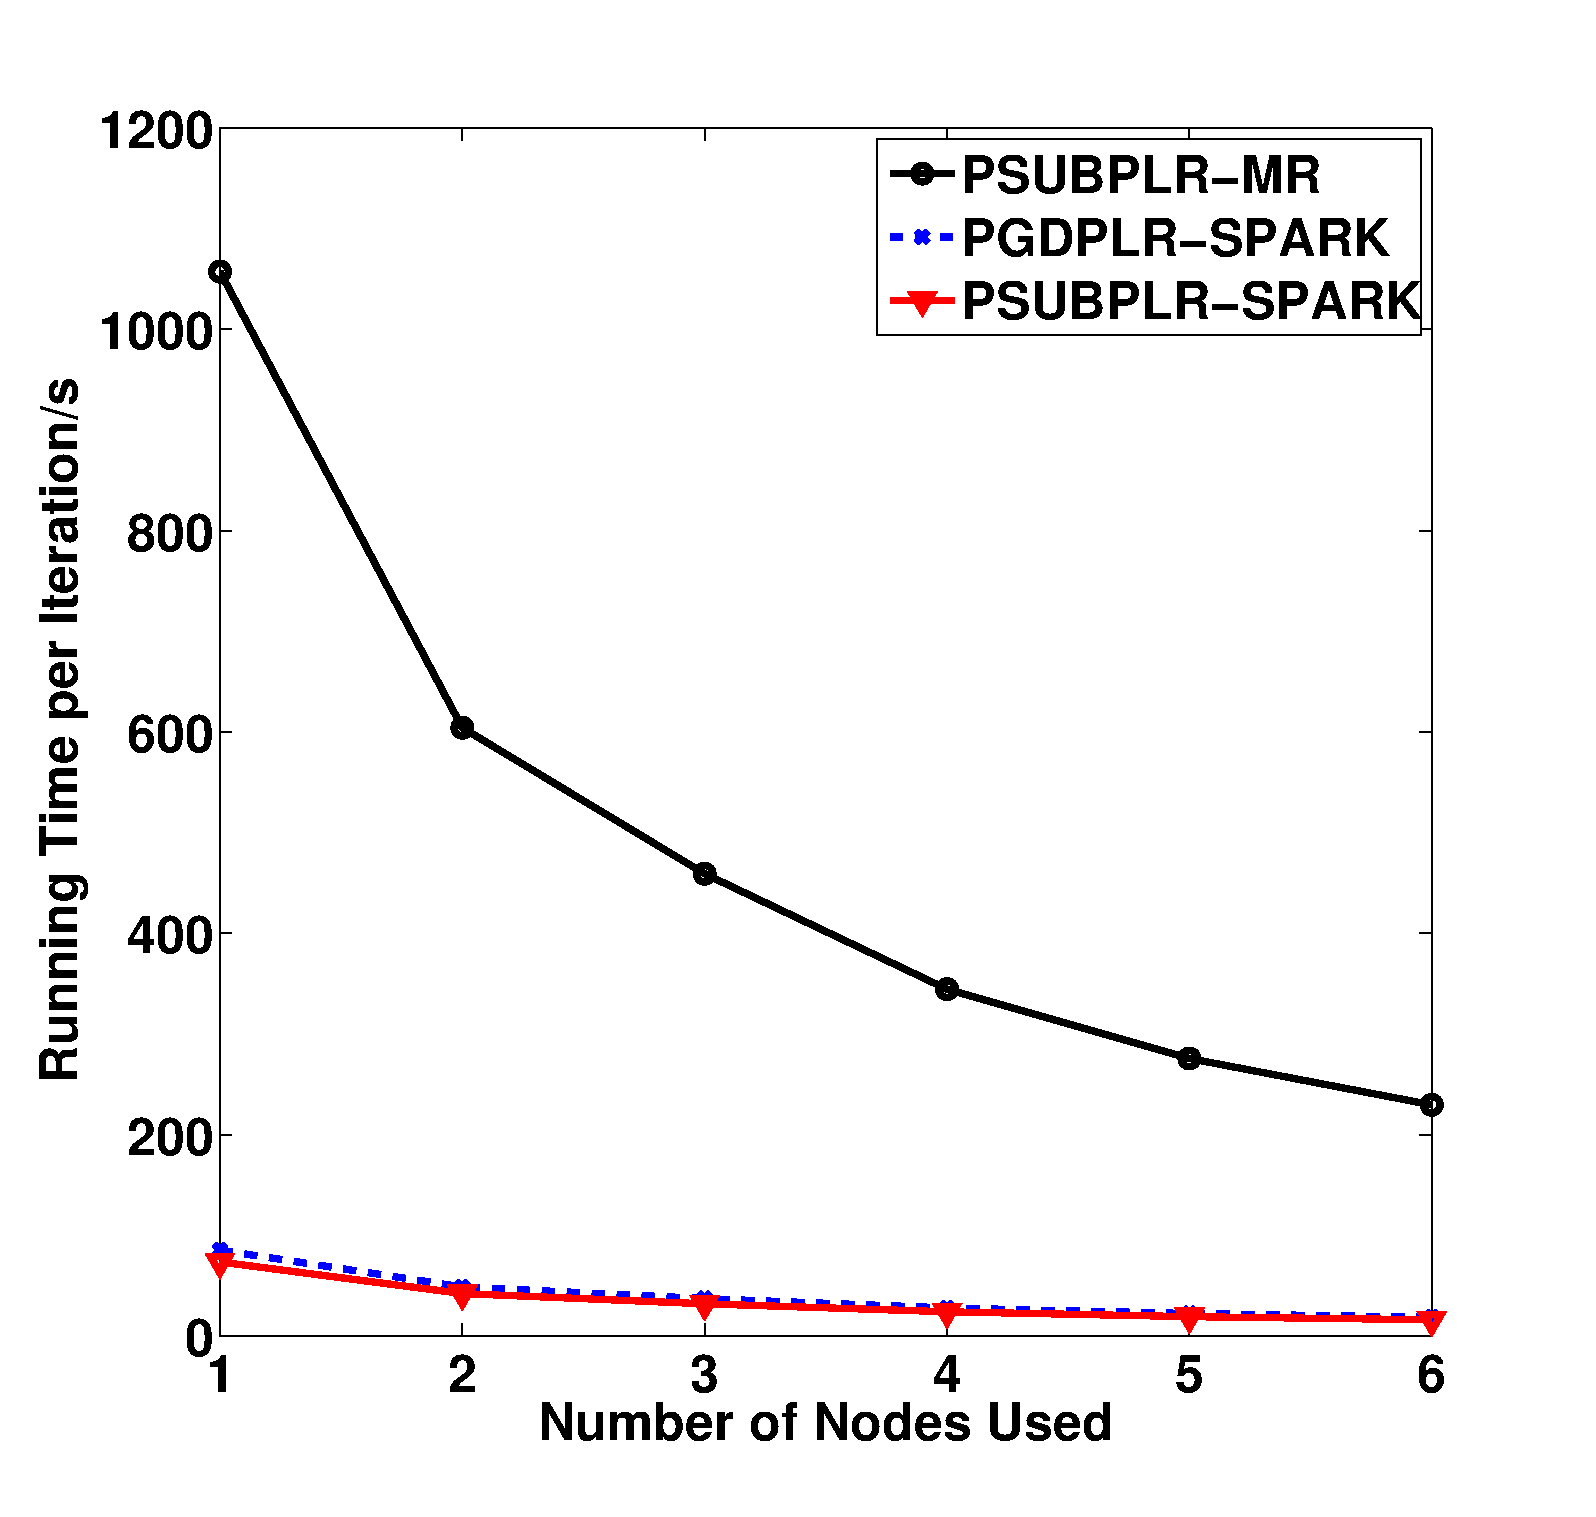
\includegraphics[height=3.9cm,width=4.5cm]{img/ECUESpam_time.eps}&
   \hspace{-0.6cm}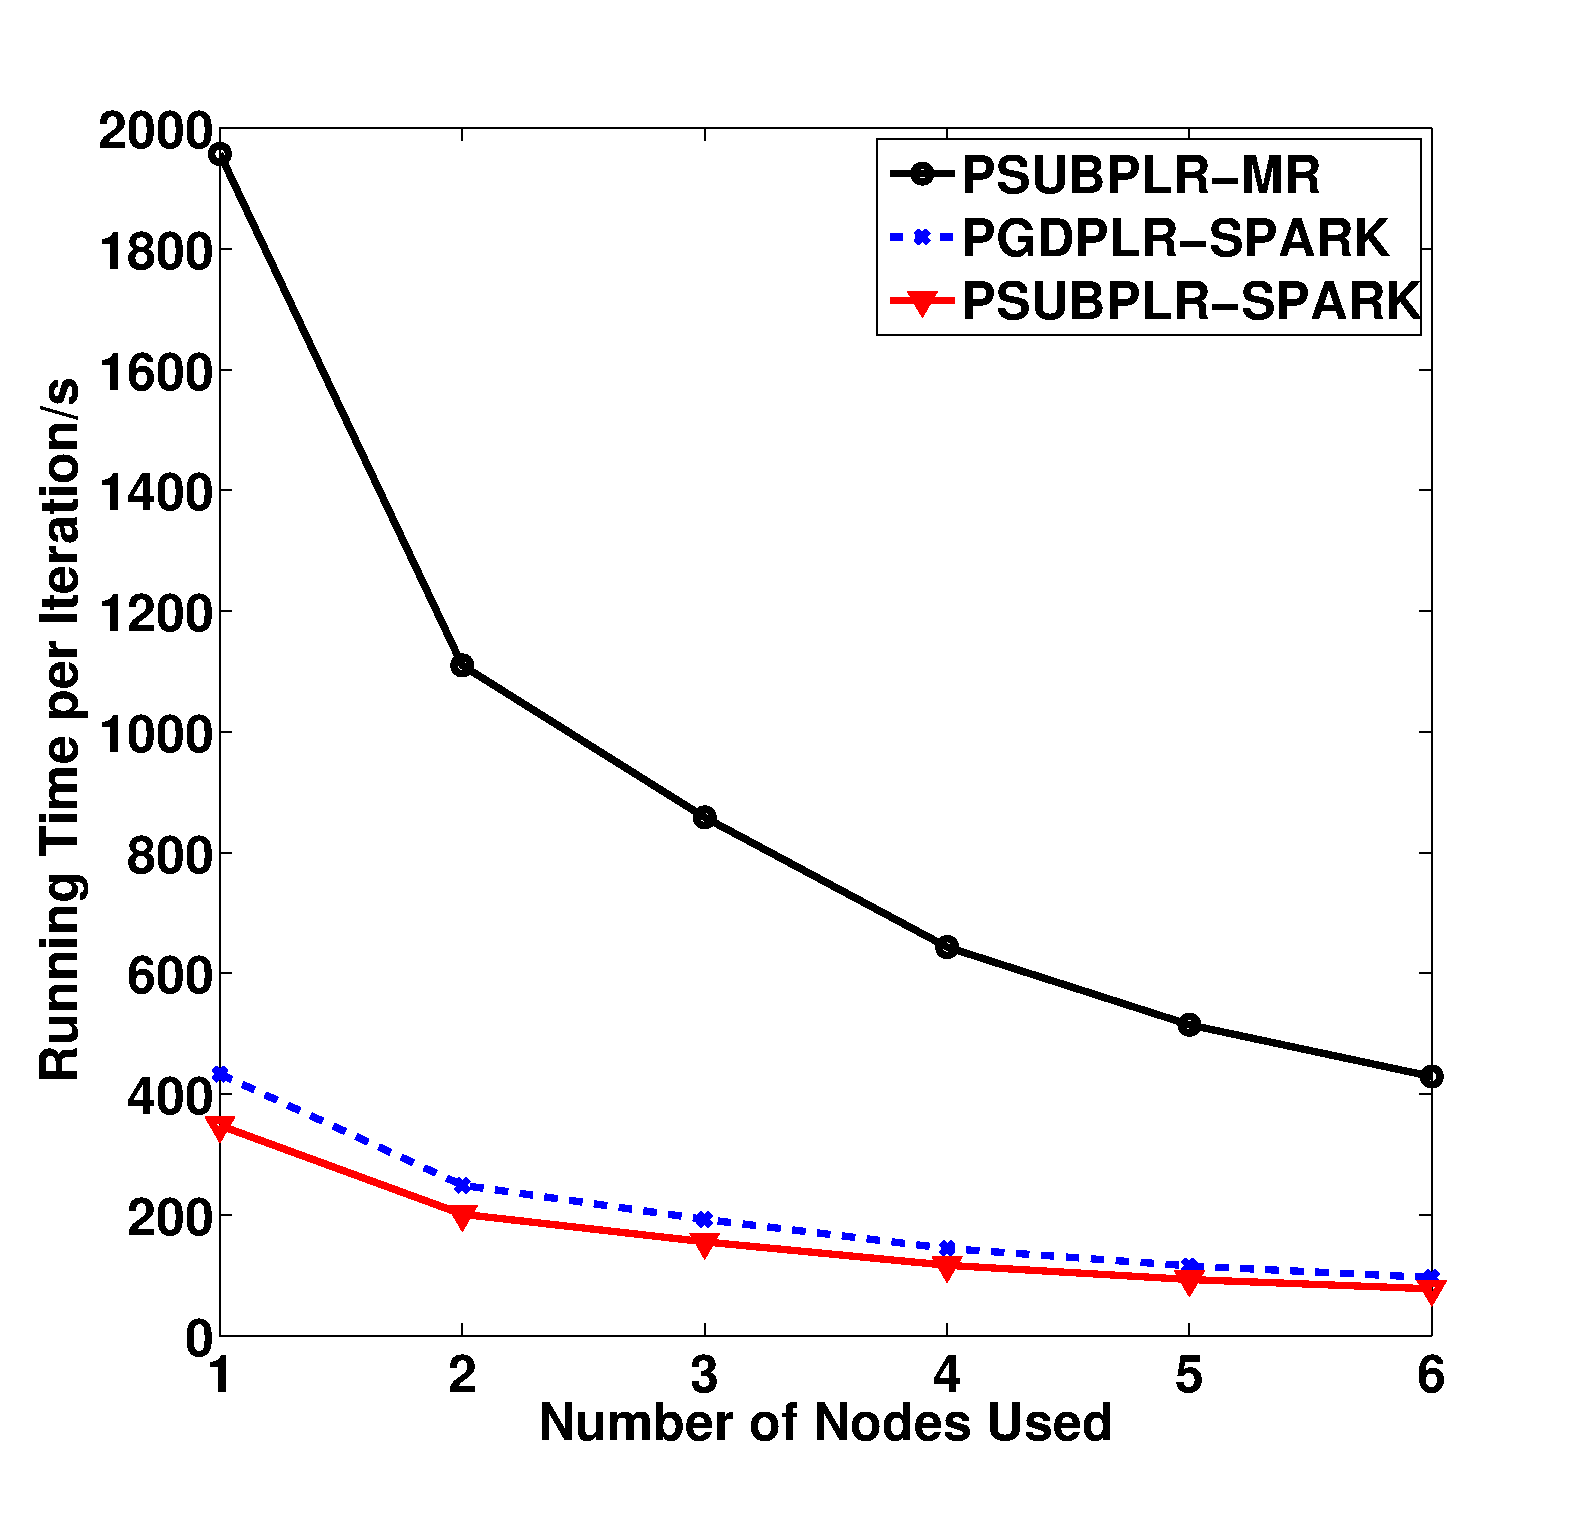
\includegraphics[height=3.9cm,width=4.5cm]{img/URL-Reputation_time.eps}\\
   (a) \textbf{20NewsGroup}. & \hspace{-0.3cm}(b) \textbf{Gisette}. & \hspace{-0.3cm}(c) \textbf{ECUESpam}. & \hspace{-0.3cm}(d) \textbf{URL-Reputation}.\\
   \end{tabular}
\end{center}\vspace{-0.3cm}
   \caption{Running time, as a function of used node number.}\vspace{-0.5cm}
\label{fig:time}
\end{figure*}
%
As we can see from the results, fewer computation resources provided, longer the implementation process will take.
However, this trend is not in a consistent fashion. When the number of machines gets higher, it will make the less impact.
We may reach a point for every algorithm when running time halts to decrease as machine number increases.
This shows the true scalability of the designed algorithm, which we can study in our future work.

\subsection{Fault Tolerance}
There are both system level techniques and algorithm level techniques to provide fault tolerance in parallel computation.
Results are shown in Table~\ref{tab:table5}.
\begin{table}[h]
\centering
\caption{Fault Tolerance Analysis}\label{tab:table5}\vspace{-0.3cm}
\begin{tabular}{|c|c|c|}
\hline
           & System Level & Algorithm Level \\
\hline
PSUBPLR-MR & \Checkmark & \Checkmark \\
\hline
PGDPLR-SPARK & \Checkmark & \XSolid \\
\hline
PSUBPLR-SPARK & \Checkmark &  \Checkmark \\
\hline
\end{tabular}
\end{table}
Here, randomization is employed in all sublinear methods, thus providing algorithm level fault tolerance for PSUBPLR-MR and PSUBPLR-SPARK.
Hadoop and Spark can both provide system level fault tolerance, but in different ways. Hadoop employs HDFS while Spark has RDDs.
Of all six test programs, PSUBPLR-MR and PSUBPLR-SPARK are fault-tolerant in both system level and algorithm level.

We show the iteration time as a function of percentage of failed maps on \textbf{URL-Reputation} dataset for all three parallel test programs in Fig.~\ref{fig:14}.
This is tested on 6 nodes.
\begin{figure}[tb]
\center 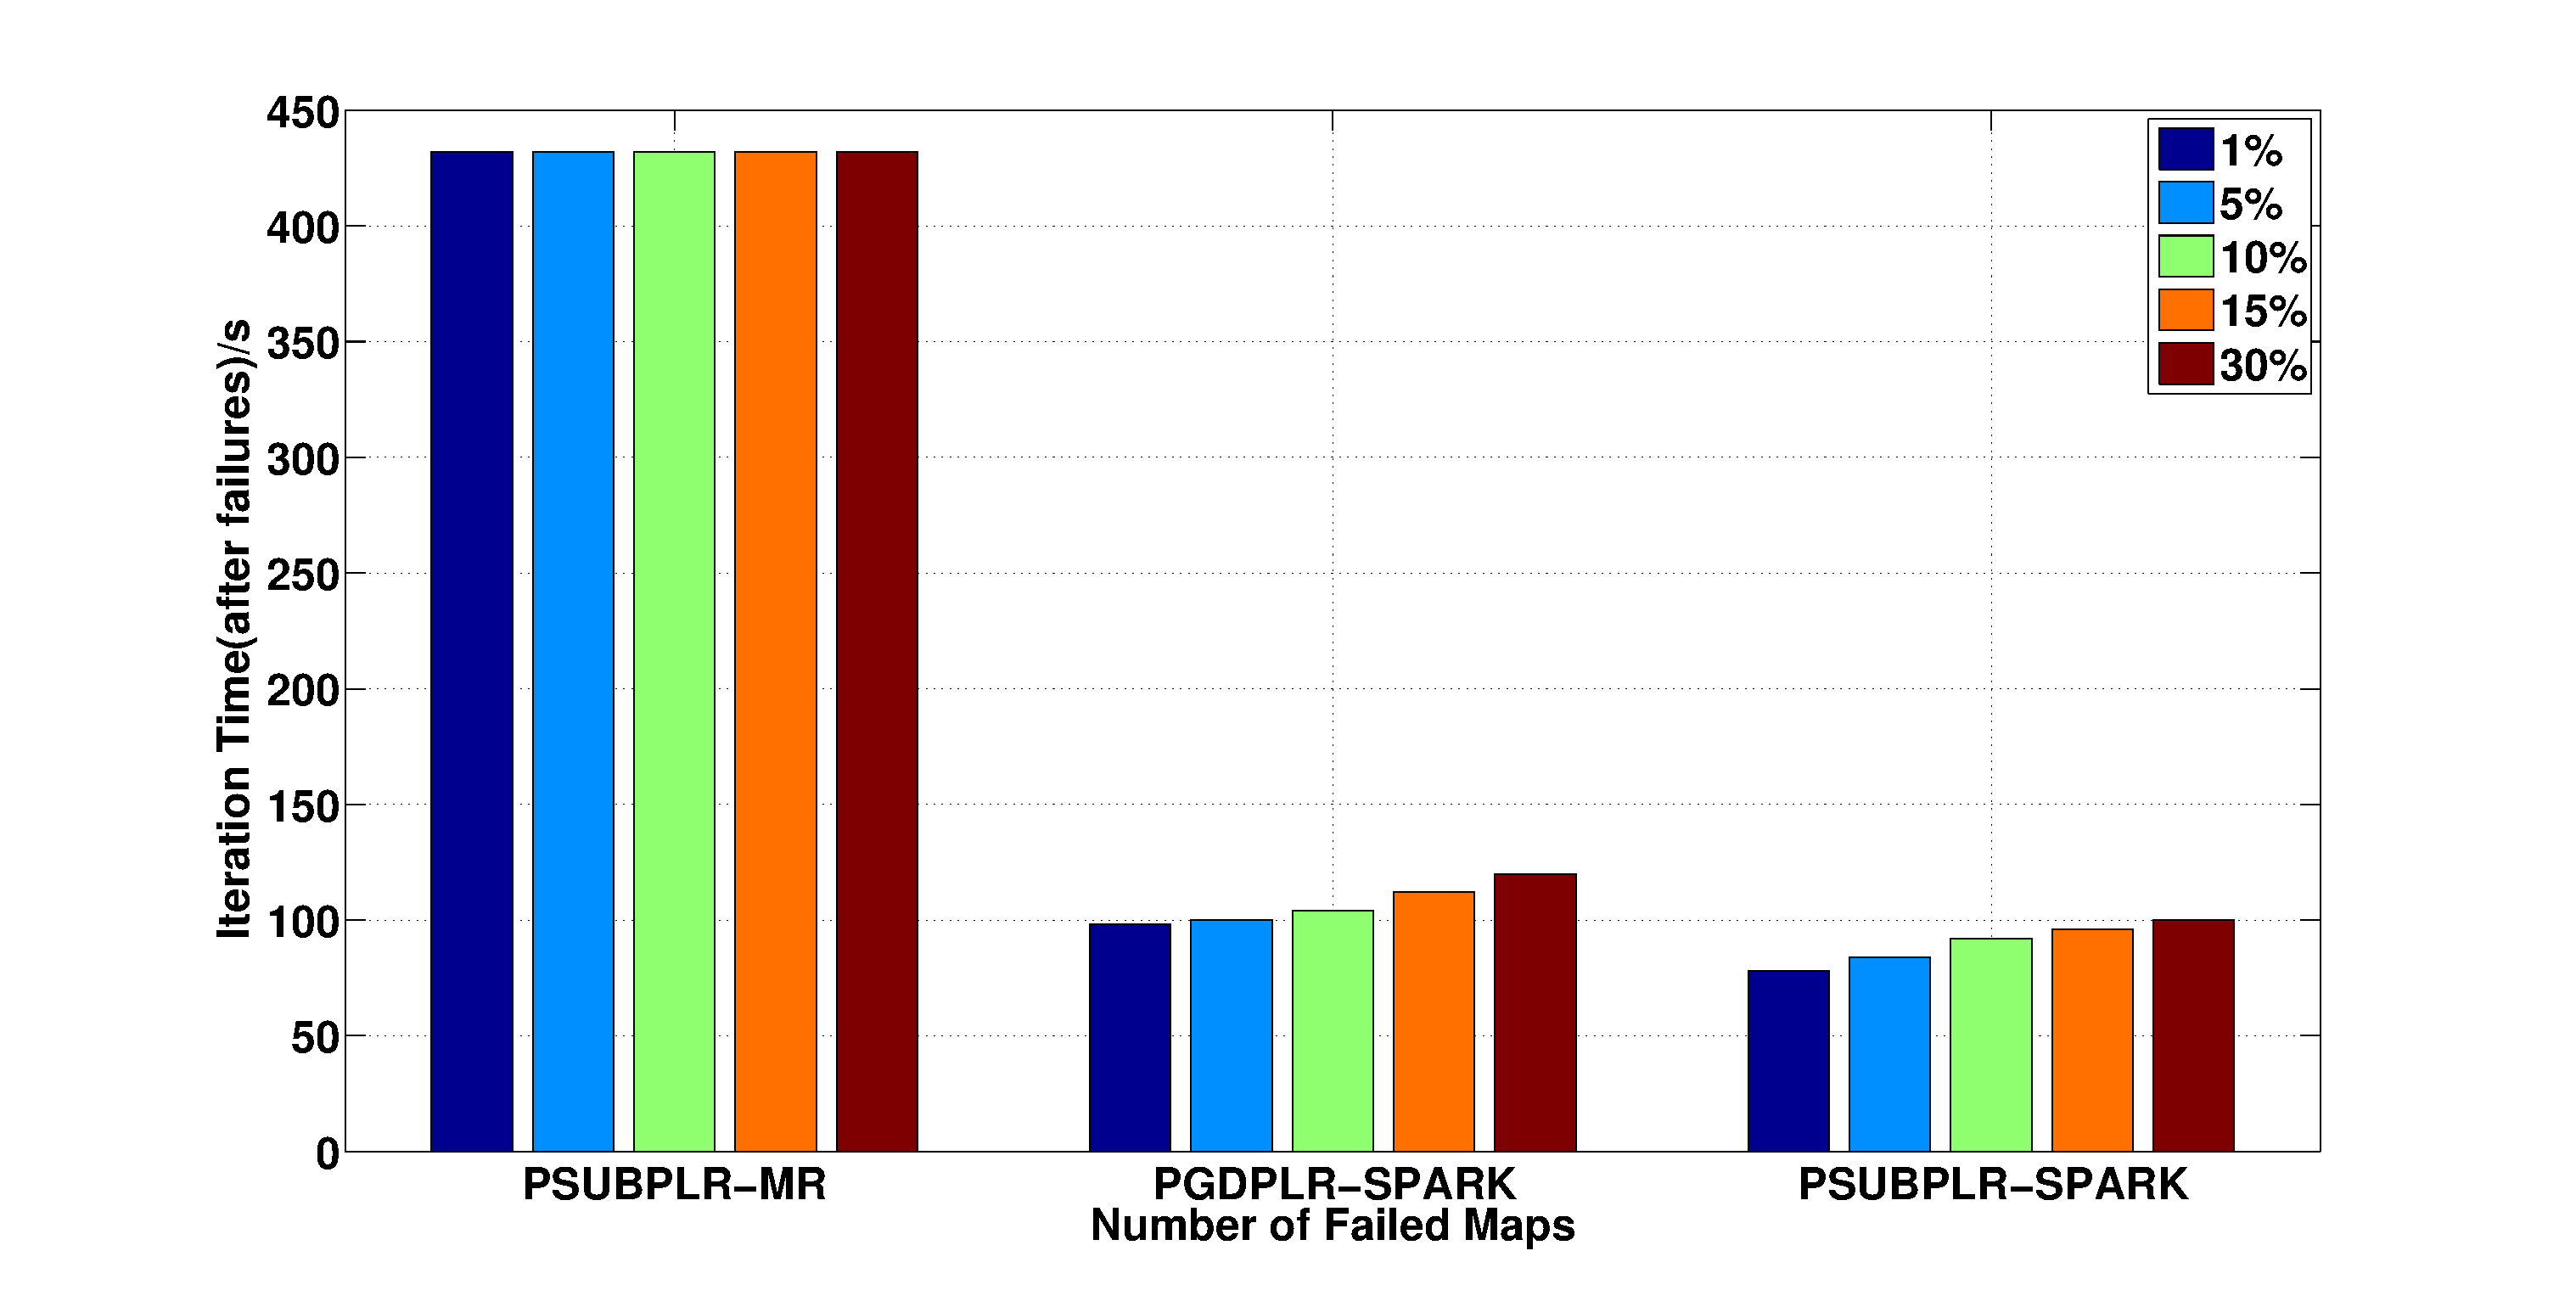
\includegraphics[height=4cm,width=8cm]{img/fault_tolerance.eps}\vspace{-0.3cm}
\caption{Iteration time, as a function of percentage of failed maps, on \textbf{URL-Reputation} Dataset, run on 6 nodes}\label{fig:14}\vspace{-0.5cm}
\end{figure}
As Fig.~\ref{fig:14} shows, iteration time of PSUBPLR-MR remains unaffected when maps fail. But it takes the cost of precision loss if we enforce that no additional iterations are implemented.
PGDPLR-SPARK and PSUBPLR-SPARK will increase iteration time when the maps fail. It is due to RDD reconstruction. The increase is not significant.
This difference also reveals the different mechanism of fault tolerance between Hadoop and Spark.

\section{Conclusion} \label{sec:concl}
In this paper we analyzed three optimization approaches along with two computing platforms to train LR model on large-scale, high-dimensional datasets for classification. A novel parallel sublinear algorithm for LR implemented on both Hadoop and Spark is presented. Based on extensive experiments, we summarized key features of each algorithm implemented on different computing platforms.
We can conclude that sequential algorithms with memory intensive operations like Liblinear can perform very well if datasets can fit in memory.
For massive datasets, if limited by machine resources, Mahout with its online algorithm is a good choice with a slightly lower precision.
If machine resources are abundant, as Spark outperforms Hadoop for LR model training, we recommend choosing between parallel sublinear method and parallel gradient descent method (both on Spark) to trade off between speedup and precision.

In future work, we will continue to explore the situations of even bigger dataset, and extend the results to multi-calss classification models of LR. We also would like to focus on combining algorithm design and computing platforms to optimize classifiers in machine learning.

\begin{small}
\bibliographystyle{plain}
\bibliography{mlpaper}
\end{small}
\end{document}
